\chapter{基于重要性和网络拥塞的任务传输调度方案}
\label{cha:Yosemite}
传统的网络资源管理机制主要是流级别或者包级别。
最近,流组(coflow)作为一种新的并行应用数据传输通信模型而被提出。
流组(coflow)对网络资源的应用级语义进行了有效的建模,
因此可以通过将流组(coflow)作为网络资源分配或调度的基本元素来更好地实现一些高级优化目标,如减少应用的传输延迟等。
虽然有效的流组(coflow)调度方法已经被研究,本章节中,建议对coflow调度时考虑权重,
权重被用来表示不同coflows优先级或者coflow的紧急程度。
本章引入加权流组完成时间(Weighted Coflow Completion Time,简称WCCT)问题,
设计一个不需要知道流组(coflow)信息就可以进行有效调度的算法,根据权重和网络拥塞程度调度流组(coflow),
同时设计一个名为Yosemite的调度算法,并通过数据中心的真实流量对Yosemite进行仿真评测。
评估结果显示,与最新的coflow调度算法相比,
Yosemite可以使得平均WCCT减少超过$40\%$,
对于重要性在平均以上的coflow,
coflow的平均完成时间减少超过$30\%$的。
和最有效的coflow调度方法相比,
WCCT优化性能大约提高了$30\%$,对于重要性在平均以上的coflow,
平均完成时间减少大约$25\%\sim30\%$。

\section{概述}
目前,数据中心很多实时的应用需要低延迟\cite{Latency,mastrolilli2010minimizing}和高吞吐量\cite{CloudMirror},
例如那些使用map-reduce计算模型的密集型计算应用\cite{dean2008mapreduce},以及那些使用分布式文件存储\cite{lin2012secure,dimakis606049decentralized}系统等。
为了满足这些要求,数据中心网络基础设施已经专门的定制和改进,
在拓扑设计,路由方案以及传输优化方面付出了巨大的努力。

在已有的各类成果中,流级别调度方法试图根据相应流的特征调度到达的流的数据包。
例如,PDQ\cite{PDQ}和pFabric\cite{pFabric}实现最短工作优先(Shortest Job First,简称SJF)策略,以使短流抢占长流的带宽。
因此,流平均完成时间(Average Flow Completion Time,简称AFCT)减少,应用程序的传输延迟降低。
但是,对于分布式应用包括很多并行的数据流,单条数据流的传输完成,并不能代表应用传输的完成,
当并行数据流均传输完成时,才算传输完毕。
因此只对单条流的传输优化,而不考虑它们之间的相互关系,
应用的整体传输性能可能无法有效改善,甚至可能受到影响。


最近,流组(coflow)作为一种新的并行应用数据传输通信的抽象模型而提出。
coflow是两组机器之间流的集合,这些数据流具有相近的语义和类似的目标\cite{chowdhury2012coflow}。
例如,最小化集合中最慢的流的完成时间,或者确保集合中的流满足共同的期限。
流组(coflow)对网络资源使用的应用级语义进行了有效的建模,
因此可以通过将coflow作为网络资源分配或调度的基本元素来更好地实现高级优化目标,如减少应用程序的传输延迟。
 
 最近很多成果已经研究了用于最小化流组(coflow)完成时间(Coflow Completion Time,简称CCT)的高效coflow调度方法。
 Varys \cite{chowdhury2014efficient}提出了最小有效瓶颈优先(Smallest- Effective-Bottleneck-First,简称SEBF )启发式算法来确定coflow的调度顺序,
 并使用最小化期望分配带宽(Minimum-Allocation-for-Desired-Duration,简称MADD)来计算要分配的带宽。
然而,Varys是一种智能程度很低的调度,它依赖于调度器得知流信息(如流大小或流到达时间)来决定如何调度流组(coflow)。
这些限制会限制Varys在实际中的使用和部署。
为了解决这个问题,新的一些研究比如Aalo\cite{chowdhury2015efficient},Barrat\cite{dogar2014decentralized},sunflows\cite{huang2016sunflow}和CODA\cite{zhang2016coda}可以不用预先得知coflow的信息(流大小或流到达时间)对coflow进行智能调度。
 
在本文中,对coflow的调度进行进一步的深入研究,建议对coflow赋予权重,
分配给coflow的权重来表示coflow的优先级或者coflow应用的优先级。
事实上,在实际中,应用有不同的重要性或者优先级,
例如,分布式搜索应用的内部传输的数据流比支持分布式存储系统上的文件备份的数据流更为重要。
当调度两个应用程序的coflow时,需考虑coflow的重要性。
为此,给coflow分配不同的权重,即搜索引擎的coflow具有较高的权重,而文件备份的coflow具有较低的权重,
的优化目标是最小化coflow的加权完成时间之和。

将非抢先式调度算法\ref{IWCCM-offline}改成不需要预先得知coflow信息的在线调度方案。
在线算法Yosemite存在较小的性能损失,但可以在线调度coflow,而不必事先知道coflow的大小或者到达时间。
通过使用数据中心真实流量来仿真和测试评估来测试Yosemite的性能,并将其与具有最佳已知性能的最新的coflow调度算法(如Varys \cite{chowdhury2014efficient},Aalo \cite{chowdhury2015efficient}和Barrat\cite{dogar2014decentralized}进行对比。
结果表明,Yosemite在降低加权混合完成时间方面表现相当好。
本章节做了以下工作:

(1)提出使用权重coflow作为数据中心资源调度的管理方案来给应用分配资源。
从一个中型数据中心收集实际应用的流量,并深入分析权重coflow调度的必要性和重要性。


(2)评估coflow的各个调度策略并与最新的不用预先得知coflow的信息调度的算法对比。
使用真实的数据中心流量评估并且测试Yosemite,评估结果发现,Yosemite可以减少超过$40\%$的WCCT。
此外,对于超过平均水平的coflow而言,Yosemite可以减少平均完成时间大约$30\%$。
和当前最有效的不可预知coflow进行调度的方法相比,
Yosemite 分别减少了约$30\%$的平均WCCT和对紧急程度在平均值以上的coflow的$20\%$$\sim$$30\%$的完成时间。

\section{研究动机和相关工作}\label{Yosemite-motivation}
数据中心现在正成为托管大量服务和应用程序的重要基础设施。
为了满足数据中心中应用对高吞吐量带宽和低延迟的需求,大量的研究工作致力于网络资源分配和调度。
例如,DCTCP\cite{DCTCP},D$^2$TCP\cite{D2TCP},L$^2$DCT\cite{L2DCT},LPD\cite{LPD},D$^3$\cite{D3}和PDQ是流级别的速率控制或调度方案,
这些方案侧重于优化流的完成时间,或者满足流对期限的要求。

Coflow的概念最近已经被提出\cite{chowdhury2012coflow},以满足更高层次应用对性能要求。
其中coflow是具有相同的语义和共同目标的两组机器之间的流集合。
当前业界关心最小化coflow平均完成时间。
特别是,Varys是基于网络瓶颈进行的优化,Varys使用最小瓶颈优先的启发式算法来决定coflow的优先级,最终优化coflow的平均完成时间。
而D-CLAS\cite{luo2016towards},Aalo\cite{chowdhury2015efficient},sunflows\cite{huang2016sunflow}和CODA\cite{zhang2016coda},
试图“猜测” coflows的一些特性,智能化的对coflow进行调度。
前者被称为“白盒”方法,因为这种方法需要预先得知coflow的大小,宽度的一些信息,
后者被称为“黑盒”方法,因为调度时,不需要提前得知coflow的信息,系统会自动的获取和识别这些信息。


虽然这些coflow级别的调度方法确实提高了通信传输的性能和效率,但是这些方法把coflow都看作同样重要。
coflow或者应用之间调度的性能差异取决于不同的调度策略。
例如,有的调度方案倾向于短的coflow优先,有的调度方案倾向于宽的coflow优先,不同的方案达到不同的调度效果。
从此角度,认为coflow或者应用是有优先级,当调度coflow或者应用时,优先级应该被考虑进去。
例如,分布式搜索应用的内部传输的数据流,比支持分布式存储系统上的文件备份的数据流更为重要。
当前对coflow的调度策略,主要侧重根据coflow的宽度和长度对coflow进行优化,应用的重要性和coflow的长度以及宽度是没有相关关系。
因此,当前出现的很多调度算法,并不能满足coflow调度的核心需求。
\begin{table}[h]
\centering
\footnotesize
 \caption{数据中心的应用和它们的紧急程度} \label{Yosemite:measure}
\begin{tabular}{|c|c|c|c|c|c|} \hline
\toprule
App Name  & Type &  width&  length (MB)&Emergence Level\\
\midrule
Event &     communication    &20&5     &  significant \\
vRouter &  communication     &8&3 &  significant\\
Druid&     interactive   &6&18   &  important \\
Hadoop&  computation  &5&42     &  normal \\
Web&     interactive   &3&5     &  normal\\
VoltDB&     background  &4&21    &  normal\\
Hive&     background   &7&32     &  unimportant \\
Redies&    background   &2&30    &  unimportant \\
data-backup&    background   &3&124     &  lax \\
data-dist& background      &5&93  &lax \\
\bottomrule
 \end{tabular}
 \end{table}
 
 
 \begin{table}[!htb]
\centering
\footnotesize
 \caption{Hadoop内部的coflow和它们的重要性} \label{Yosemite:measure2}
\begin{tabular}{|c|c|c|c|c|c|} \hline
\toprule
Coflow Type  &  width&length (MB)&Emergence Level\\
\midrule
index-sort    &10&3  &significant \\
db-analysis   &3&12     &  important \\
index-count   &6&20 &  normal\\
log-analysis   &6&31   &  unimportant \\
crawler  &4&12     &  unimportant \\
word-count  &3&11     &  unimportant\\
   \bottomrule
 \end{tabular}
 \end{table}
 
 
为了说明数据中心内coflow重要性应该被考虑,对来自一个中型的数据中心的流量进行测量和分析,
假设数据中心中有3000台机器,同时并行了100个应用程序。
在和数据中心管理人员以及网络工程师进行深入讨论以后,深入分析了从60个机架中收集的720个服务器的流量信息。
流持续1个月左右,表\ref{Yosemite:measure}显示的是最常用的前10个应用的信息。
把应用分成5个重要级:紧急的应用,重要的应用,正常的应用,不重要的应用和松散的应用。
例如,事件程序产生的流量和vRoute应用程序产生的路由信息流量,具有最高的优先级。
而数据备份和数据分发是在后台运行的应用程序,产生的是背景流量,背景流量的优先级较低。
看到,应用的数据流小或者包含更宽的流,并不代表具有更高的优先级。
例如,Hive(平均宽度是7)比Web(平均宽度是3)的宽度大,但Hive比Web的优先级低。
另一个例子是Web(平均长度是5MB)的平均长度比Druid(平均长度是18MB)小,但是Web的优先级比Druid低。
这支持了前面的观点,即一般情况下,应用的coflow的紧急程度和宽度以及长度没有必然的关联。
表\ref{Yosemite:measure2}进一步显示了hadoop应用中不同coflow的细节,从中可以得出类似的结论。
例如,word-count(平均宽度是3)比index-count(平均宽度是6)的宽度小,优先级低。
另一个例子是log-analysis(平均宽度是6)的平均长度比db-analysis(平均宽度是3)大,但是优先级低。
这支持了前面的观点,即一般情况下,应用的coflow的紧急程度和宽度以及长度没有必然的关联。
\begin{figure}[h]
  \centering%
  \subcaptionbox{平均CCT} %标题的长度,超过则会换行,如下一个小图。
    {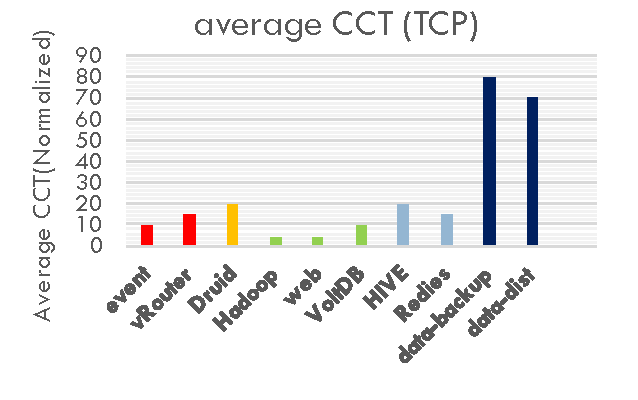
\includegraphics[width=0.5\columnwidth]{figures/Yosemite/figs/motivation/motivation_color_1.pdf}}%
  \subcaptionbox{平均CCT(使用Varys)}
      {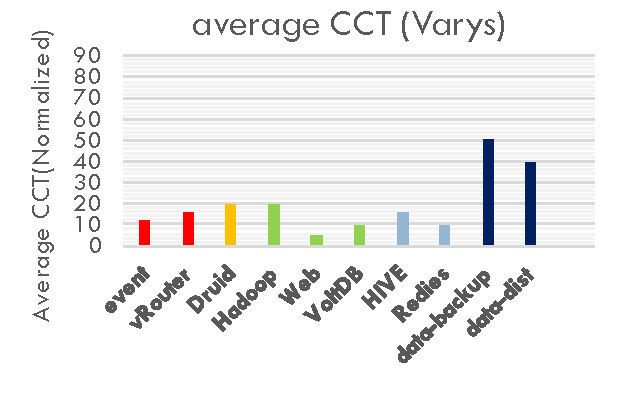
\includegraphics[width=0.5\columnwidth]{figures/Yosemite/figs/motivation/motivation_color_2.pdf}}
  \subcaptionbox{Hadoop CCT}%标题的长度,超过则会换行,如下一个小图。
    {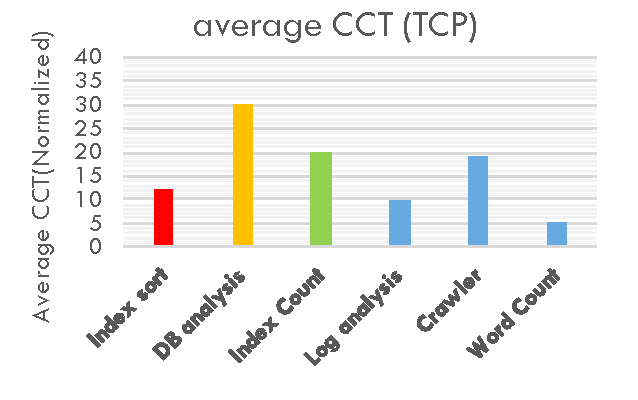
\includegraphics[width=0.5\columnwidth]{figures/Yosemite/figs/motivation/motivation_color_3.pdf}}%
  %\hspace{7em}%
  \subcaptionbox{Hadoop CCT(使用Varys)}
      {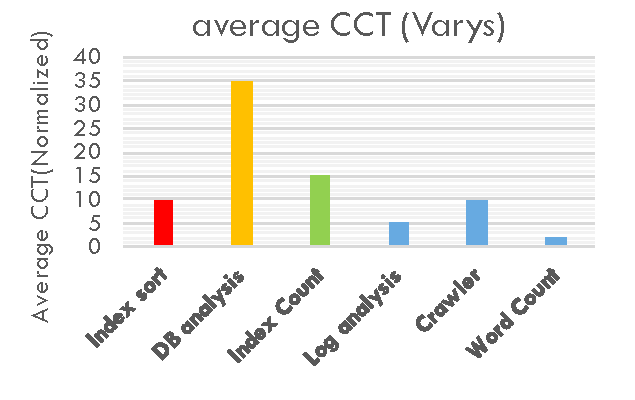
\includegraphics[width=0.5\columnwidth]{figures/Yosemite/figs/motivation/motivation_color_4.pdf}}
  \caption{平均Coflow完成时间,coflow根据紧急程度进行分类}
  \label{Yosemite_Motivation_fig1}
\end{figure}


\begin{figure}[h]
\centering
\subcaptionbox{Coflow同时到达端口}
 {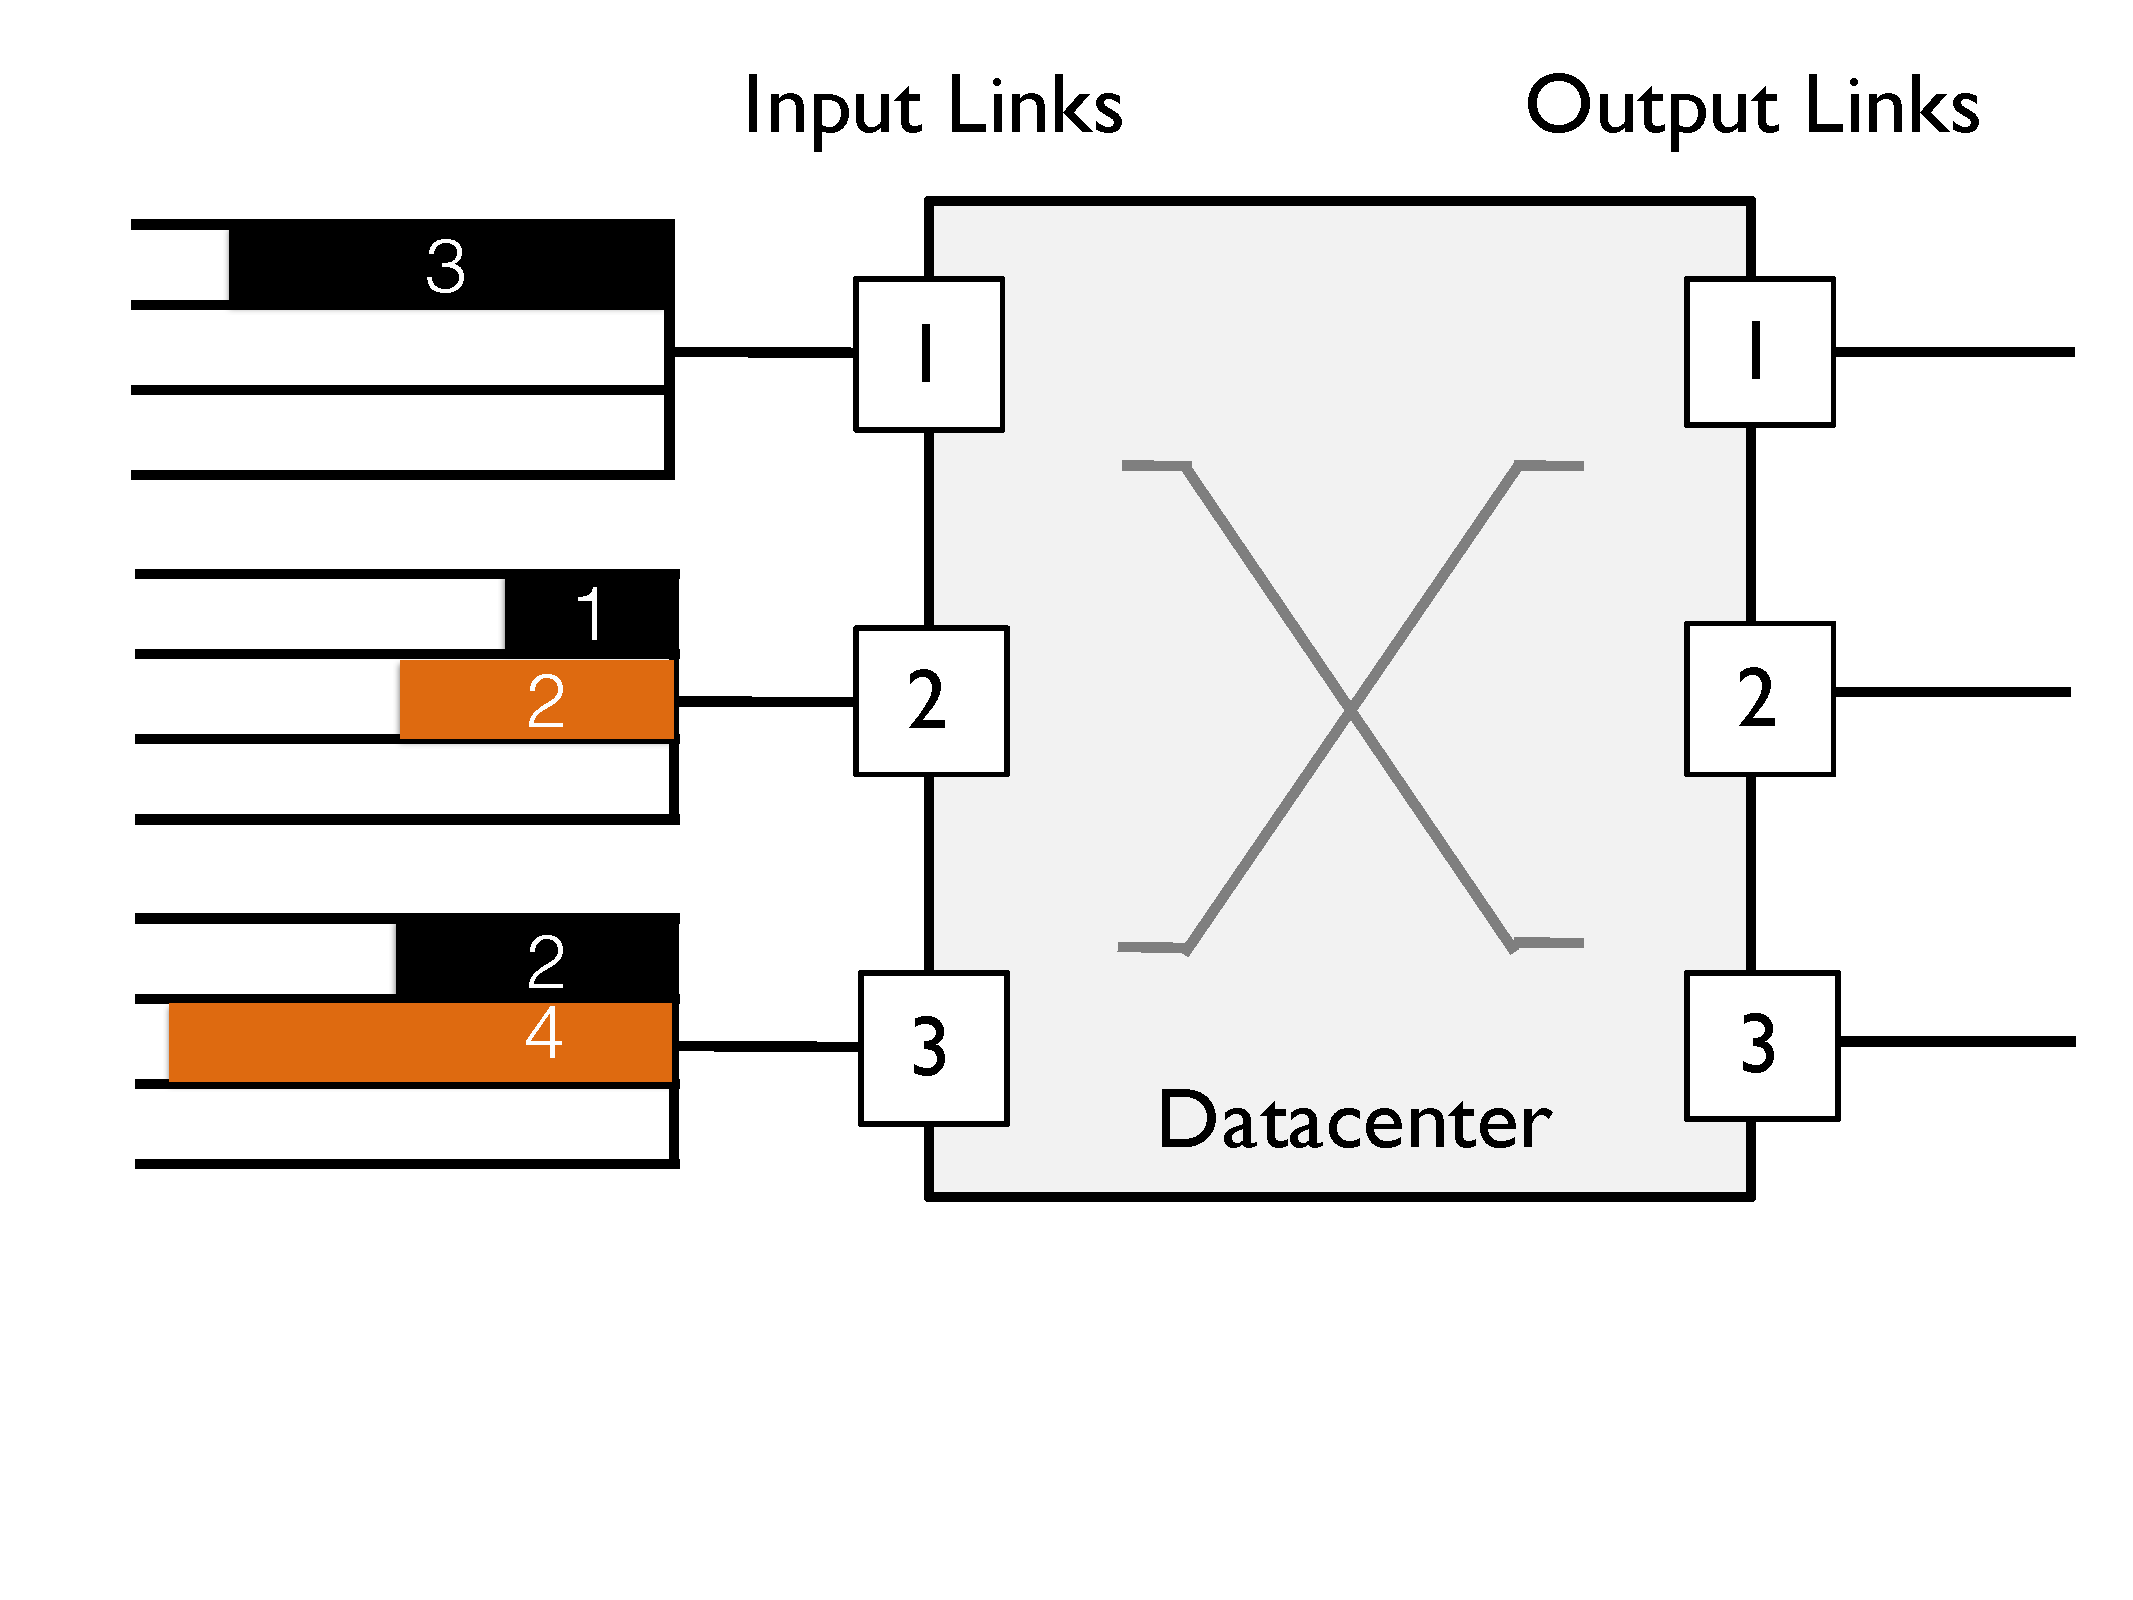
\includegraphics[width=0.32\columnwidth]{figures/Yosemite/figs/motivation/motivation_color_5.pdf}}
\subcaptionbox{使用TCP进行调度}
{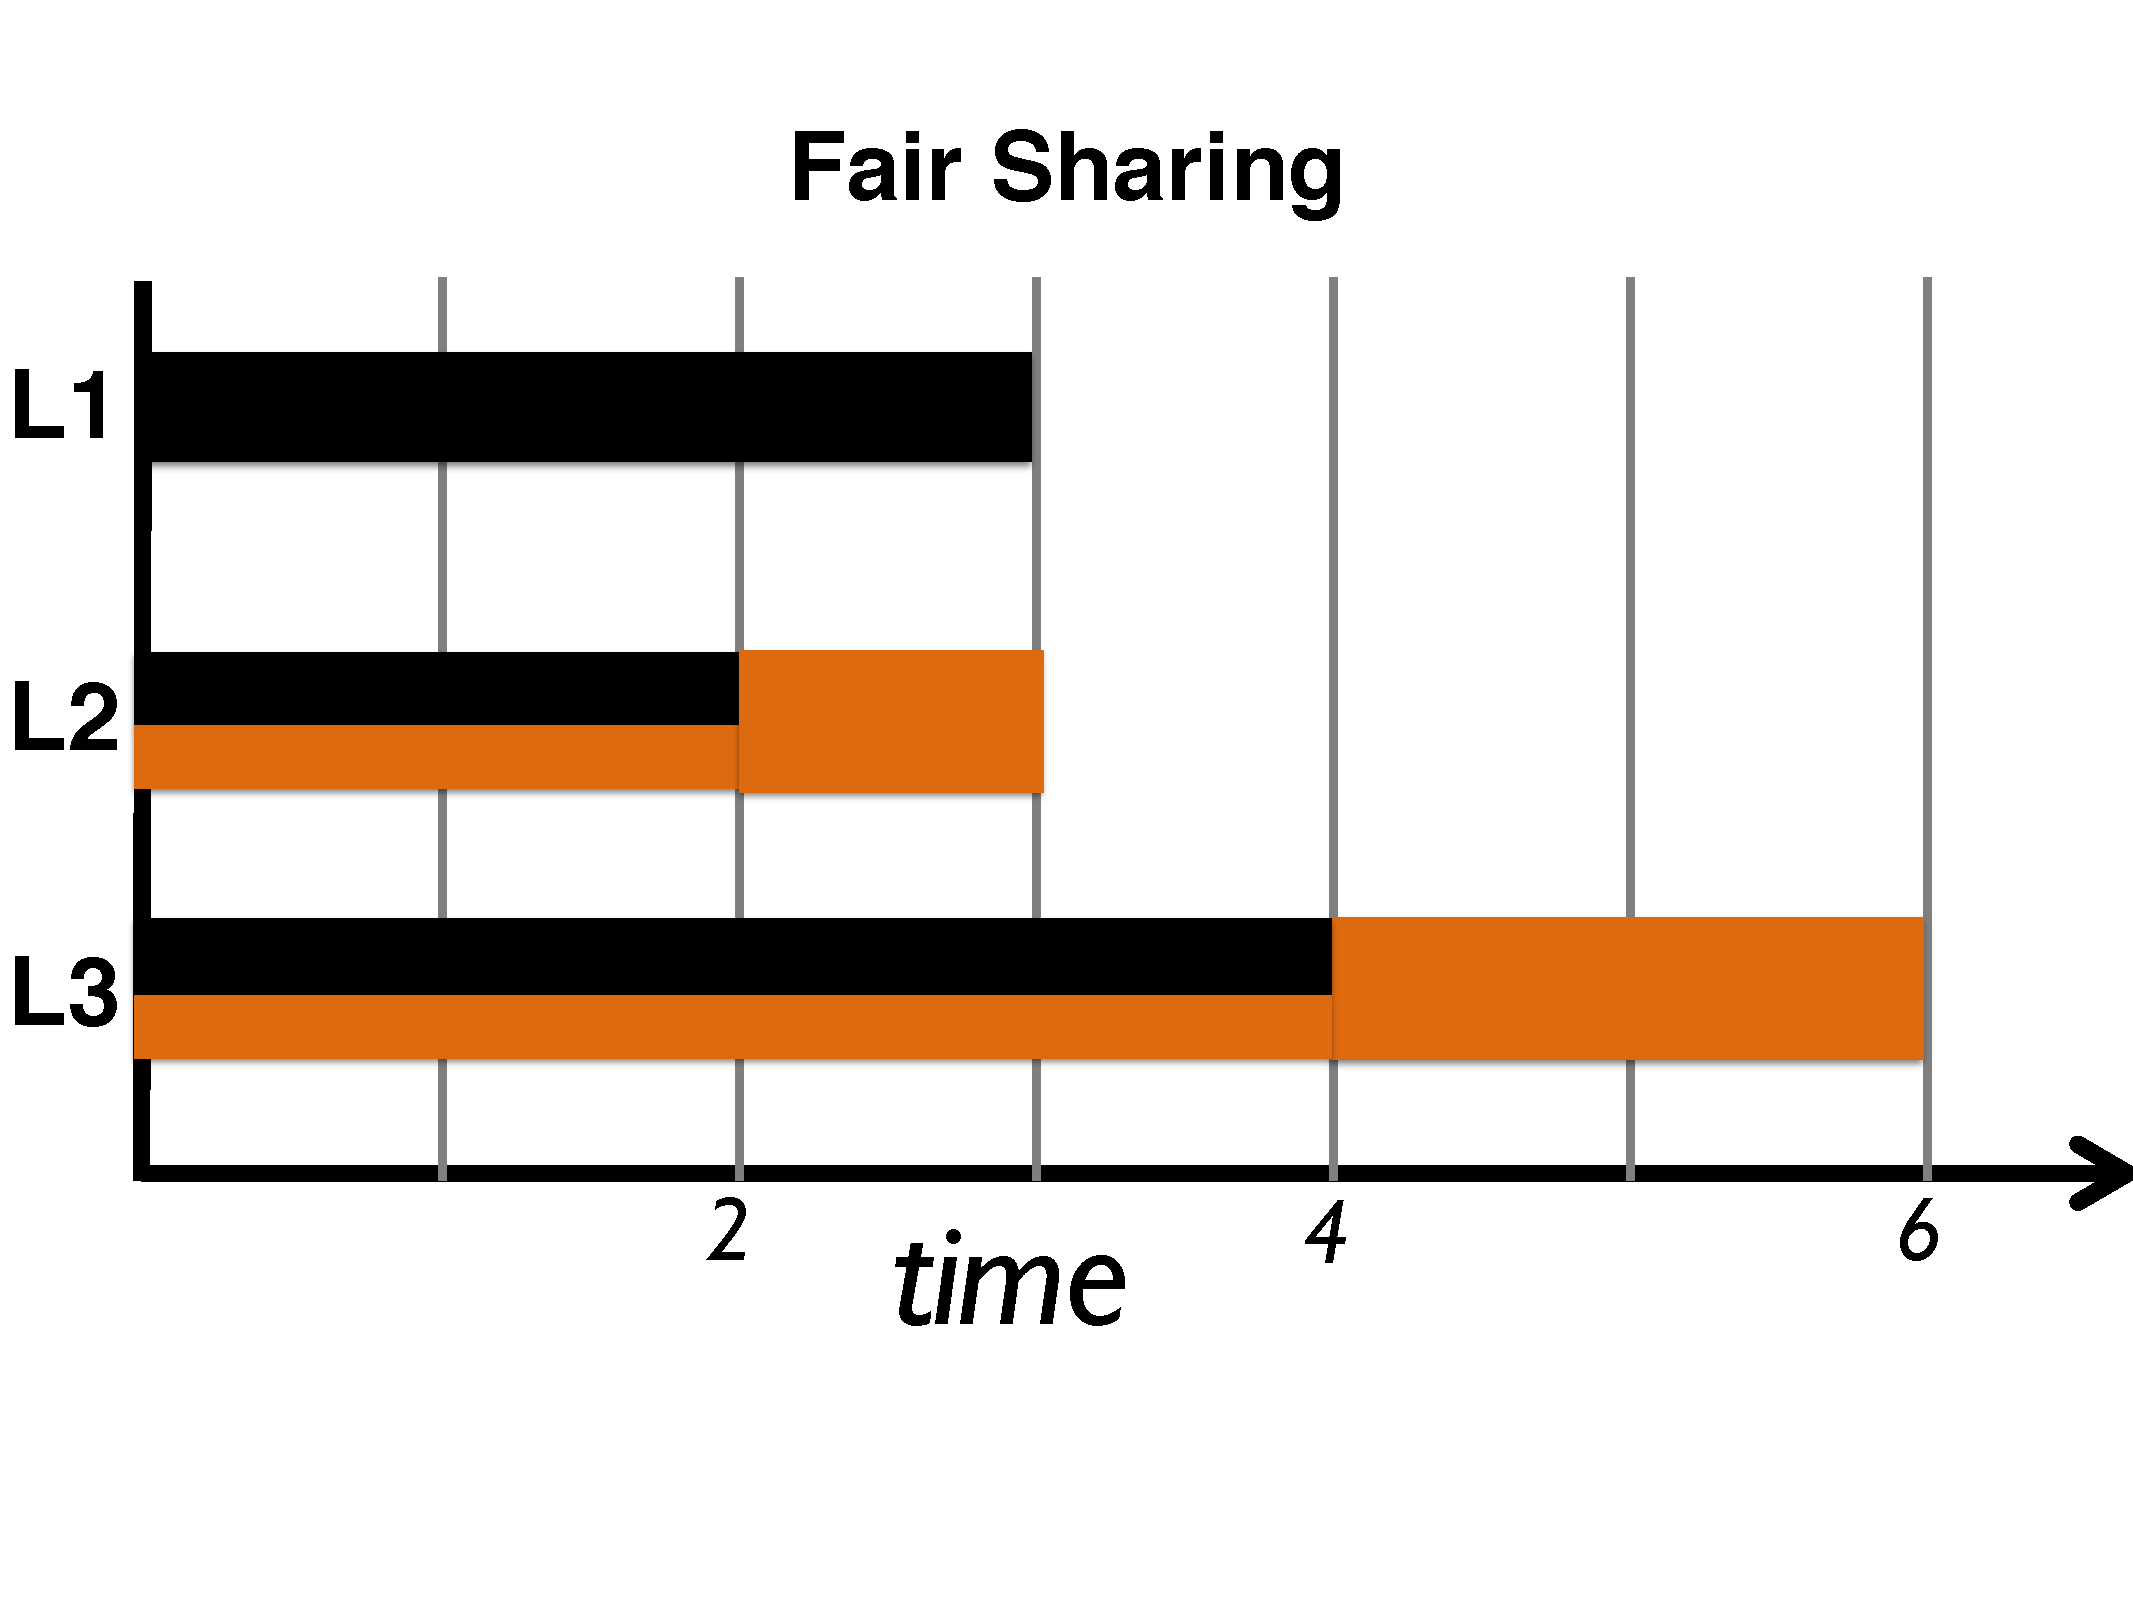
\includegraphics[width=0.32\columnwidth]{figures/Yosemite/figs/motivation/motivation_color_7.pdf}}
\subcaptionbox{使用Varys进行调度}
{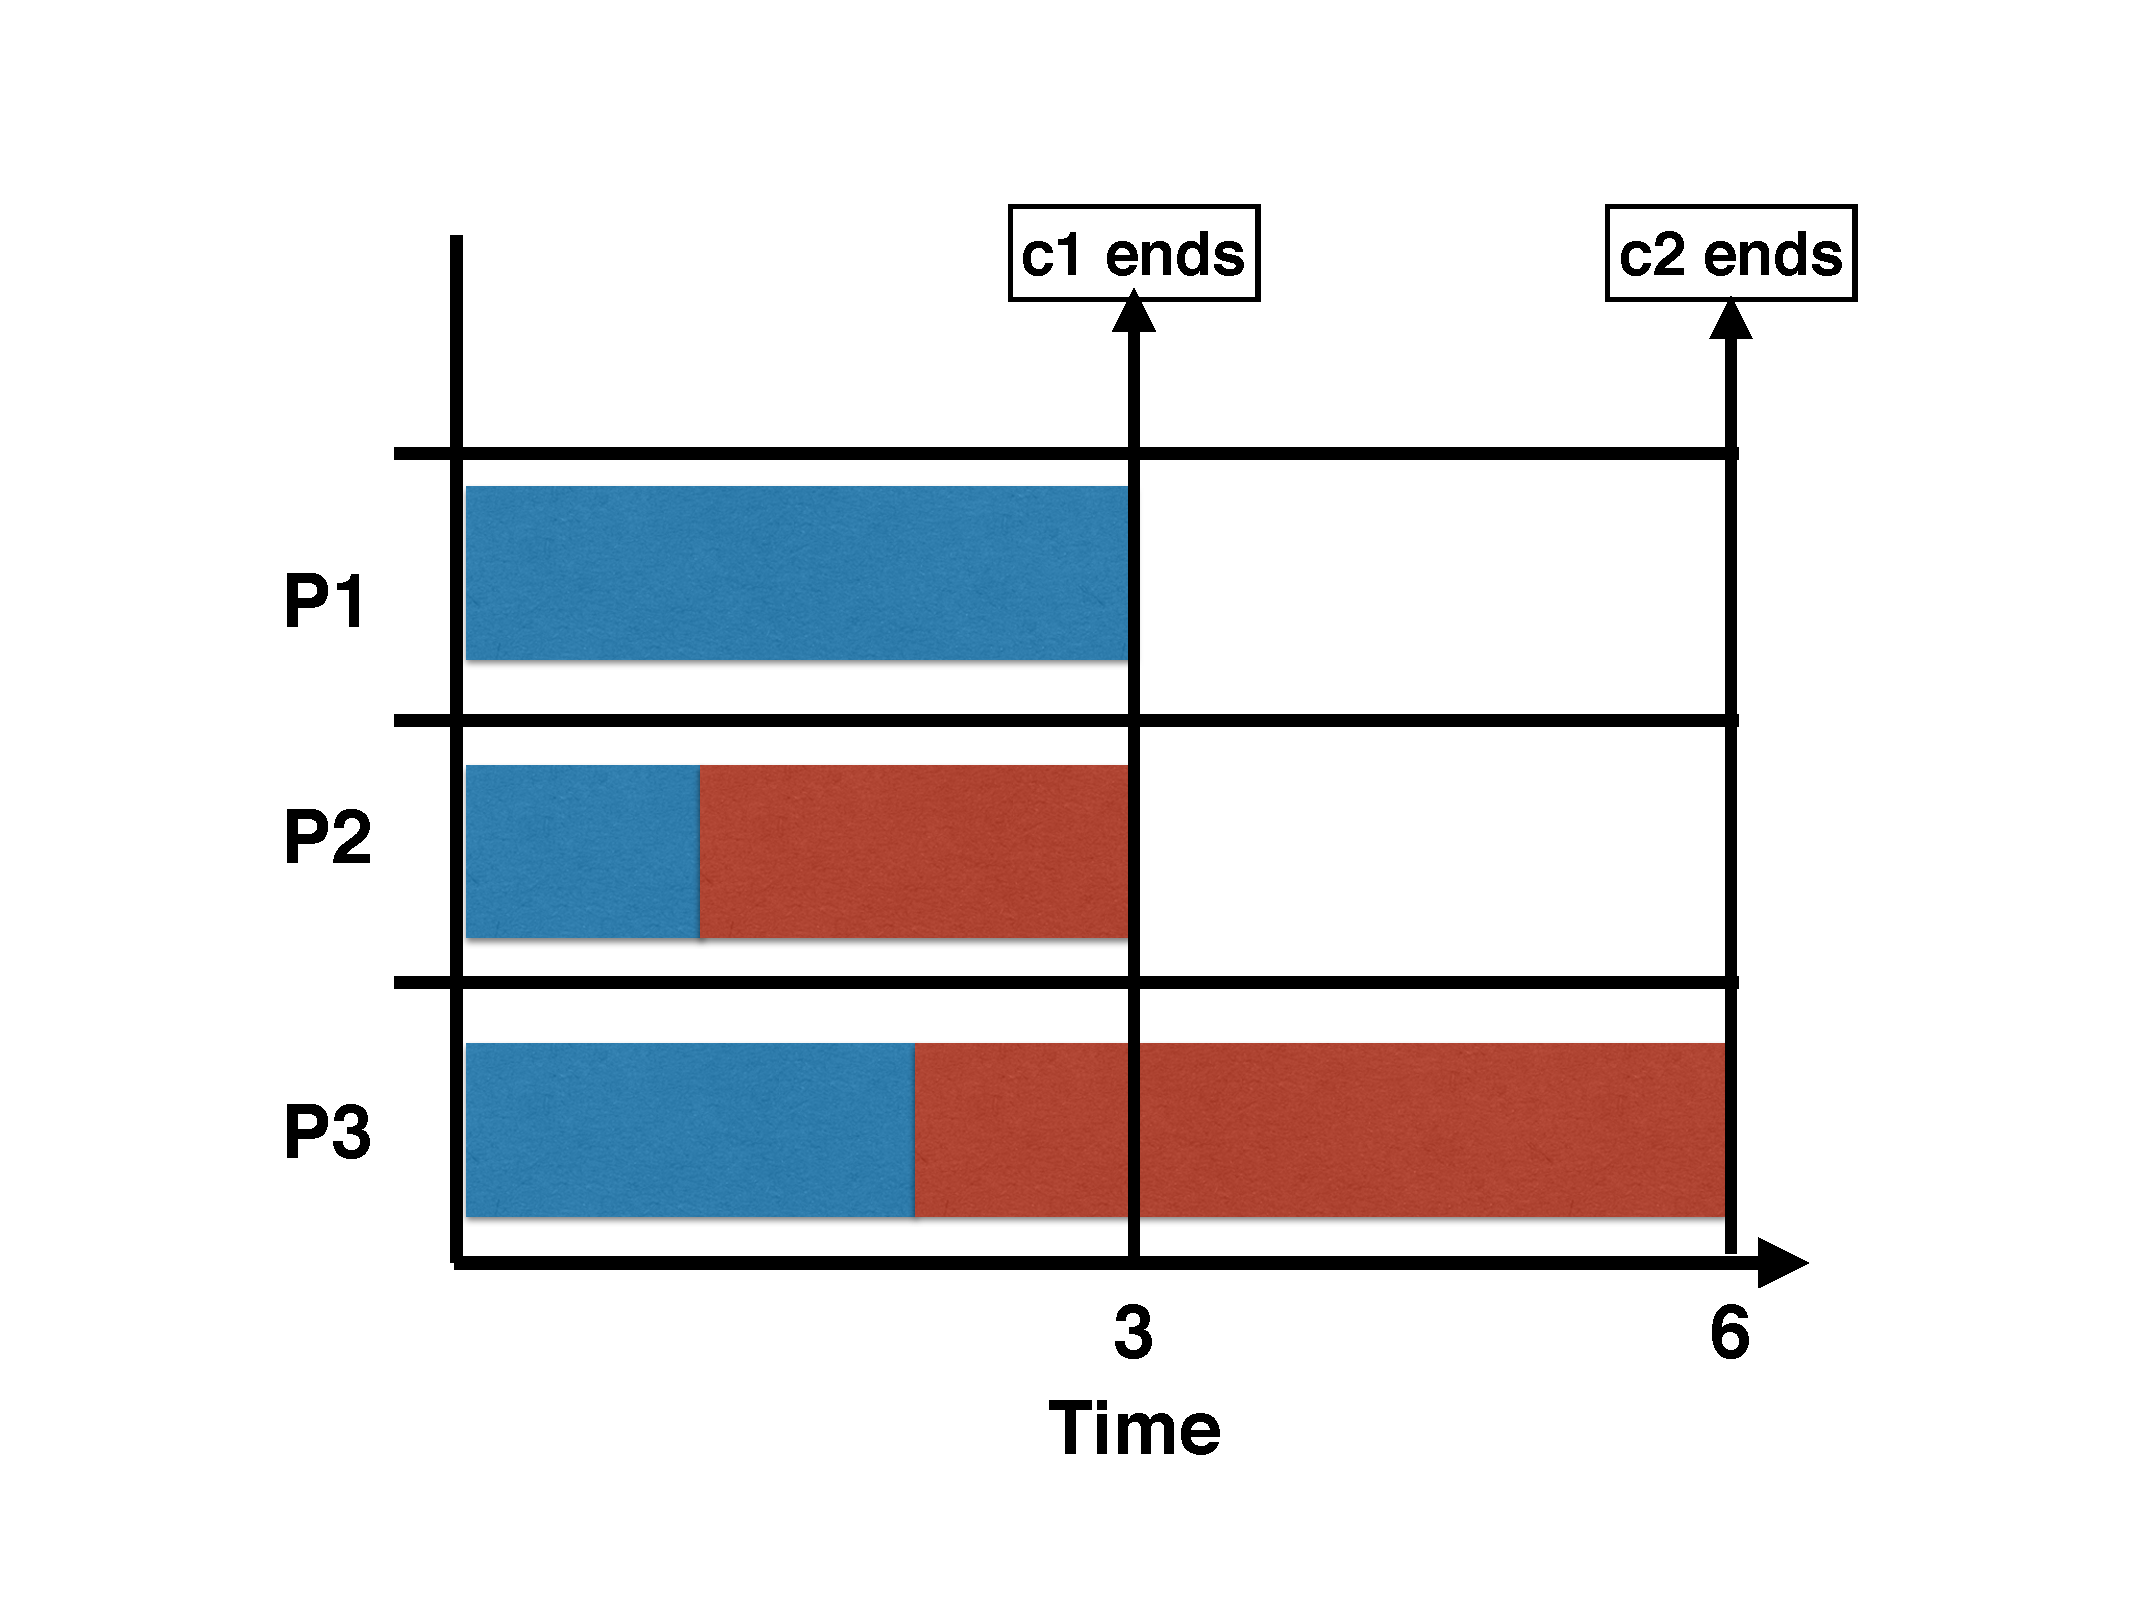
\includegraphics[width=0.32\columnwidth]{figures/Yosemite/figs/motivation/motivation_color_6.pdf}}
\caption{两条coflow同时到达端口,coflow $cf_1$(蓝色)包含3条流,coflow $cf_2$(红色)包含两条流。 $cf_2$的优先级比 $cf_1$高}
\label{Yosemite_Motivation_fig2}
\end{figure}

为了说明现有的coflow调度方法的无效性,
绘制了不同coflows的平均Coflow完成时间(CCT),按照紧急程度进行,如图\ref{Yosemite_Motivation_fig1}所示。
图\ref{Yosemite_Motivation_fig1}(a)显示了所有应用在使用TCP的情形下平均Coflow完成时间(CCT)。
可以看到,对于紧急的应用Event和vRouter,平均CCT是9,11。
Druid的紧急程度是重要,平均CCT是20。
Hadoop,web,VoltDb的紧急程度是正常程度,平均流组完成时间是6,7,10。
Hive,Redies的紧急程度是不重要,平均流组完成时间是20,15。
data-dist和data-backup的紧急程度是松散,平均流组完成时间是80,70。
而图\ref{Yosemite_Motivation_fig1}(b)显示了使用Varys进行调度时的仿真结果。
对于紧急的应用Event和vRouter,平均CCT是11,15。
Druid的紧急程度是重要,平均CCT是21。
Hadoop,web,VoltDb的紧急程度是正常程度,平均流组完成时间是20,5,9。
Hive,Redies的紧急程度是不重要,平均流组完成时间是12,10。
data-dist和data-backup的紧急程度是松散,平均流组完成时间是50,40。
通过比较图\ref{Yosemite_Motivation_fig1}(a)和图\ref{Yosemite_Motivation_fig1}(b),
可以看到,对于紧急程度是紧急和重要的应用,Varys对平均完成时间基本没有提高,甚至对于Event,使用Varys,平均流组完成时间甚至增大。
Varys对于紧急程度为正常,不重要和松散的应用提高幅度较大。

图\ref{Yosemite_Motivation_fig1}(c)显示的是对于Hadoop应用使用TCP的情形下平均流组完成时间(Coflow Completion Time,简称CCT)。
可以看到,对于紧急的应用Index Count,平均CCT是12。
DB Analysis的紧急程度是重要,平均CCT是35。
Log analysis,crawler,word-count的紧急程度是不重要,平均CCT是10,20,5。
而图\ref{Yosemite_Motivation_fig1}(d)显示了使用Varys对Hadoop应用进行调度时的仿真结果。
对于紧急的应用Index Count,平均CCT是10。
Druid的紧急程度是重要,平均CCT是21。
Hadoop,web,VoltDb的紧急程度是正常程度,平均CCT是5,10,3。
通过比较图\ref{Yosemite_Motivation_fig1}(c)和图\ref{Yosemite_Motivation_fig1}(d),
可以观察到和图\ref{Yosemite_Motivation_fig1}(a),图\ref{Yosemite_Motivation_fig1}(b)类似的效果。

为了分析上述问题出现的原因,展示了一个小的调度实例,如图\ref{Yosemite_Motivation_fig2}所示。
在这个实例中,如图\ref{Yosemite_Motivation_fig2}(a)所示,两条coflow,$cf_1$和 $cf_2$同时到达端口,
$cf_1$有3条子流,$cf_2$有2条子流,$cf_2$的优先级比$cf_1$高。
图\ref{Yosemite_Motivation_fig2}(b)展示的是使用TCP作为调度协议的结果,图\ref{Yosemite_Motivation_fig2}(c)展示的是使用Varys作为调度方法的结果。
可以发现,相对于TCP,更加紧急的$cf_2$完成时间未变,而$cf_1$减小了1。
分析出现这个问题的原因是Varys使用\textbf{Smallest-Effective-Bottleneck-First }(SEBF)但是忽略了coflow的重要性。
这提示,在调度应用的数据任务时,coflow的重要性应该也被考虑,使用权重表示coflow的重要性,优化目标位平均权重完成时间。


%\section{模型和问题定义}
%
%在这部分,假设网络是非阻塞的,体系结构,如图\ref{erasure-non-blocking-fig}所示,
%在本体系结构下,拥塞只发生在入端口和出端口,中间路径是没有拥塞发生的。
%在这个模型上,考虑coflow问题的定义,
%随后,定义Idealized Weighted Coflow Completion Time Minimization (IWCCTM) 问题,并分析这个问题的复杂性。
%
%\subsection{问题定义}
%考虑在数据中心中调度 $n$ 条coflow,假设网络是一个非阻塞的结构,
%这个结构有$m$台主机,意味着在这个结构中有$m$入端口和$m$个出端口。
%一个coflow定义为数据流的集合,这些数据流有共同的目标,比如最小化最最慢的流完成时间,或者共同需要满足共同的期限等。
%coflow的定义为$F^{(k)}=\{f^k_{i,j}|1 \leq i\leq m,1\leq j \leq m\}$,$k$是分配给coflow的序号,$f^k_{i,j}$是每条流的长度(标准化后),这条流是从
%机器$i$到机器 $j$。因为每个端口的转发能力是1,所以,当只有这一条coflow进行传输时,传输时间是$f^k_{i,j}$ 。
%如果从机器$i$到$j$没有数据传输,那么$f^k_{i,j}=0$。在本部分的讨论中,首先假设所有的coflow同时到达,随后,把这个假设去掉,
%然后讨论在线调度方法。
%使用 $w_k$表示coflow的权重,权重在实际当中可以表示为coflow $F^{(k)}$的重要性,因此完成时间$C_k$的优化可以考虑和权重相关。
%然后定义如下的 Idealized Weighted Coflow Completion Time Minimization (IWCCTM) 问题:
%
%\begin{eqnarray}
%& {\rm minimize} & \sum_{k=1}^{n} w_{k} C_{k} \label{eq:WCCO-SC} \\
%& {\rm s.t.} &\forall k,j:  \sum_{\forall l:C_l \leq C_k}\sum_{i=1}^{m}f_{i,j}^{(l)} \leq C_k  \label{eq:ingress_constraint}\\
%&&\forall k,i: \sum_{\forall l:C_l \leq C_k}\sum_{j=1}^{m}f_{i,j}^{(l)} \leq C_k   \label{eq:egress_constraint}
%\end{eqnarray}
%
%的目标是最小化权重coflow 完成时间之和,(\ref{eq:ingress_constraint})和(\ref{eq:egress_constraint})是因为入端口和出端口有带宽的限制。
%对于一个coflow $F^{(k)}$,完成时间是$C_k$,考虑在$F^{(k)}$完成之前的coflow的集合:$F^{(l)}$:$C_l \le C_k$。
%对于任意的入端口 $i$ (或者出端口$j$),在这个端口上的所有流的传输时间,至少为:$\sum_{j=1}^{m}f_{i,j}$ (出端口 $j$上的为:$\sum_{i=1}^{m}f_{i,j}$),这个值应该小于$C_k$。
%
%
%考虑一下这个问题的简化版本,希望最小化在一条链路上竞争带宽的流的总完成时间。
%众所周知,\emph{shortest job first }(最短作业优先)是最优非抢先调度策略,而\emph{short remaining time first} (最短剩余作业优先)是最优先抢占策略。
%在多链路上调度加权完成时间的问题的复杂度要高的多,正如以下命题所表明的那样。
%\subsection{NP-hard 证明}
%在本部分中,证明,在只允许非抢先调度的情形下,任务的权重完成时间之和的问题是NP-hard的。
%
% \begin{lemma}\label{IWCCTM-proof2}
% 如果只允许非抢先调度,那么IWCCTM问题和开放商店中,任务的权重完成时间之和的问题是等价的,问题的复杂度是NP-hard。
%\end{lemma}
%
%\begin{proof}
%开放商店可以被描述为:有一系列的机器 $M = \{1,...,m\}$,每台机器能执行一种类型的操作,
%任务集合表示为$N = \{1,...,n\}$,每个任务需要特定的$m$类的操作。
%每个任务 $j \in N$有一个权重$w_j \in R > 0$,并且任务$j$在机器$i$ 上的处理时间是$p_{ij} \in R\ge0$。
%当一个任务在机器上的所有操作都完成了,才能认为这个任务完成。
%特别的,一个任务的所有的操作能够并行的处理。
%
%对于一个$m \times m$的网络体系结构,一个coflow $F^{(k)}$有$2m$个子传输任务($m$ 传输任务在入端口,$m$ 个传输任务在出端口)。
%考虑开放商店中有$n$ 个任务和$2m$台转发能力相同的机器,其中,每个任务需要$2m$种操作。
%每个任务和每个操作是一对一的关系,在一台机器上的操作和一个端口上的传输是一对一的关系。
%已经被证明,在开放商店中,最小化平均任务权重完成时间是NP-hard\cite{mastrolilli2010minimizing}\cite{chen2000supply}\cite{roemer2006note}\cite{Qiu2016Experimental},因此,在非阻塞的网络体系结构中对coflow的调度问题的复杂度也是NP-hard。
%\end{proof}



\section{Yosemite算法设计}
本节提出基于重要性和网络拥塞的任务传输调度方案-Yosemite,
第\ref{cha:mode-taskl}章提出的算法\ref{IWCCM-offline}中假设所有的coflow是同时到达,
并且调度器没有预先得知coflow的信息,这些理想化的假设是不现实的,
 因此在设计能够真实部署的算法时,算法应该慎重的使用。

%在本节中,首先根据文献\cite{mastrolilli2010minimizing}中提出的思想,
%提出IWCCTM问题的非抢先式调度算法,该算法是2-近似最优的。
% 然后去掉所有的coflows同时到达的假设,并且假设流的大小不可知,
% 并且导出一个信息不可知的抢先调度算法,可以以在线方式工作。 
 

%\subsection{解决IWCCM的2近似算法}
%
%
%对于在开放商店中解决任务平均权重完成时间的问题,
%当前最优的解决方法是2-近似的贪心策略\cite{mastrolilli2010minimizing,kumar2011lp}。
%因为IWCCTM问题和开放商店任务权重完成时间有很近的关系,引入一个2-近似的非抢先调度算法如算法\ref{IWCCM-offline}所示。
% 
%\begin{algorithm}
%\KwIn{Coflow 集合 $\mathcal{F}=\{F^{(k)}\}$,权重集合$\mathcal{W}=\{w_k\}$, $1 \le k \le n$; } 
%\KwOut{a permutation $\gamma$ of $\{1, \dots, n\}$;}
%$\mathcal{P} \gets \{1, \dots, 2m\}$, $\mathcal{R} \gets \{1, \dots, n\}$\;
% $L_i^{(k)}= \sum_{j=1}^mf_{i,j}^{(k)}$  for $1 \le k \le n$ and $i \le m$\;
%  $L_{j+m}^{(k)}= \sum_{i=1}^mf_{i,j}^{(k)}$ for $1 \le k \le n$ and $ j \le m$\;
% $L_p=\sum_{1 \le k \le n}L_p^{(k)}$ for each $p \in \mathcal{P}$\;
%   \For{$i$ from $n$ to $1$ }{
%   $p^*=\arg \max \limits_{p \in \mathcal{P}}L_p$\;
%    $\gamma[i]=r^*=\arg\min \limits_{r \in \mathcal{R}} w_r/L_{p^*}^{(r)}$\;
%     $\theta=w_{r^*}/L_{p^*}^{(r^*)}$\;
%     $\mathcal{R} = \mathcal{R} \setminus \{r^*\}$\;
%    $w_r = w_r-\theta \times L_{p^*}^{(r)}$ for all $r \in \mathcal{R}$\;
%    $L_p=L_p-L_p^{(r^*)}$ for all $p \in \mathcal{P}$\;
%  }
%  \textbf{return} $\gamma$;
%  \caption{解决IWCCM的2近似算法}
%  \label{IWCCM-offline}
% \end{algorithm}
% 
% 算法\ref{IWCCM-offline}的输入是coflow的集合 $\mathcal{F}=\{F^{(k)}\}$,
% 其中包含$n$条coflow,权重集合$\mathcal{W}=\{w_k\}$,
% 其中包含$n$个权重,其中,第$k-$条coflow的定义为 $F^{(k)}=\{f^k_{i,j}|1 \leq i\leq m,1\leq j \leq m\}$,
% 这条coflow的权重是$w_k$, 这个值是$\mathcal{W}$中第$k$个权重。
% 
% 算法\ref{IWCCM-offline}首先构造了一系列的端口集合 $\mathcal{P}=\{1, \dots, 2m\}$,
% 这个集合对应着非阻塞网络体系结构的$m$个入端口和$m$个出端口,行1$\sim$4,计算了每个端口的负载。
% 然后算法迭代的找出第i个循环下要调度的coflow,循环是按照倒叙进行的,
% 在每轮迭代中,首先找出负载最重的端口$p^*$,然后找到这个端口上有最小的权重和负载比的coflow,
% 然后保存这个coflow的负载到$\gamma[i]$(行 6 $\sim$ 7),
% 随后更新要调度的coflow的集合,以及要调度的coflow集合的权重,和端口的负载(行8 $\sim$ 11),
% 随后,进行下一轮的迭代。
% 
% 算法\ref{IWCCM-offline}产生 序列$\gamma$ 的复杂度是$O(n(m+n))$,
% 并且这个算法是2-近似的,因为IWCCTM问题作了一些理想化的假设,因此这个算法不能在实际当中真正的使用。
%  
%
 
 
 算法\ref{IWCCM-offline}的关键思想在于第7行,它试图在大多数加载的端口$ p^* $上优先考虑具有权重大但负载小的coflow。
 实际上,当前数据中心网络中的端口通过利用某些负载平衡技术来进行负载均衡\cite {dean2008mapreduce}。
 所以做一个忽略端口负载差异的简化,并且把权重大但负载小的coflow设置为高优先级。
 通过用这种启发式算法替换算法\ref{IWCCM-offline}中的coflow优先级设定规则,
 随后得到一个简单的离线调度算法\ref{IWCCM-offline2}。
 
 \subsection{解决IWCCM的另一个简单离线算法}
 \begin{algorithm}
\KwIn{Coflow 集合 $\mathcal{F}=\{F^{(k)}\}$,权重集合$\mathcal{W}=\{w_k\}$, $1 \le k \le n$; } 
\KwOut{a permutation $\gamma$ of $\{1, \dots, n\}$;}
$\mathcal{R} \gets \{1, \dots, n\}$\;
   \For{$r \in \mathcal{R}$}{
   $L^r=\max(\max \limits_i  \sum_{j=1}^mf_{i,j}^{(k)},\max \limits_j   \sum_{i=1}^mf_{i,j}^{(k)})$\;
   }
   \For{$i$ from $1$ to $n$ }{
     $\gamma[i]=r^*=\arg\max \limits_{r \in \mathcal{R}}w_r/L^r$\;
     $\mathcal{R} = \mathcal{R} \setminus \{r^*\}$\;
  }
  \textbf{return} $\gamma$;
  \caption{简单离线调度算法}
  \label{IWCCM-offline2}
 \end{algorithm}
 
 
 算法\ref{IWCCM-offline2}展示的是一个简单的离线调度算法。
  算法\ref{IWCCM-offline2}首先定义coflow的负载为传输最慢的coflow传输完成需要的时间。
 算法的第2行,首先计算出所有coflow的负载,因为在假设的non-blcoking结构中,
 所有端口的转发能力都是1,因此,在非强占的调度场景下,coflow的负载是最长的流的长度。
 第4$\sim$6行是对coflow进行排序,简单的离线算法把权重大但负载小的coflow设置为高优先级。
事实上, 算法\ref{IWCCM-offline2}依然假设所有的coflow同时到达,并且需要预先得知coflow的信息,
然而,在真实的环境中,coflow的到达是随机的,并且,对于一些应用如hadoop等,很难预先得知
要传输的数据流的信息,因此,实际中可以使用已发送的流的大小进行流的负载的计算,发送的数据越多,说明数据流越长,可能的负载就越大
在做出所有这些改变之后,得到在线调度算法\ref {IWCCM-online-algorithm}。


\subsection{Yosemite算法}
 
 算法\ref {IWCCM-online-algorithm}是在线的调度算法,
当一个coflow到来时,算法\ref {IWCCM-online-algorithm}被调度器调用一次。
算法\ref {IWCCM-online-algorithm}根据上面提出的优先级排序策略对coflow进行排序(行 1 $\sim$ 11)\footnote{一个coflow的集合 $\mathcal{F}$和对应调度顺序被调度器自始至终维护着,如果没有新的coflow到达,优先级排序策略会被忽略,所有的coflow的顺序保持不变。},
随后,给每条流分配带宽 (行 12 $\sim$ 19)。
最后如果有剩余带宽,分配这些剩余带宽给流,这样保证网络资源最充分的利用。

算法\ref{IWCCM-online-algorithm}不需要预先知道coflow的信息,
它动态的根据权重和网络的情形给coflow分配带宽。
事实上,算法\ref{IWCCM-online-algorithm}近似实现最短colfow优策略。
和算法\ref{IWCCM-offline2}相比,这个算法不可避免的会存在性能损失,
在后面的实验中,会介绍因为放缩而引起的性能损失。
 
   \begin{algorithm} 
  \KwIn{Coflow list $\mathcal{F}=\{F^{(k)}\}$, weight list $\mathcal{W}=\{w_k\}$, $1 \le k \le n$; } 
\KwOut{a permutation $\gamma$ of $\{1, \dots, n\}$;}
  \If{a new coflow arrives}{
 update the coflow list $\mathcal{F}=\{F^{(k)}\}$\;
  $n=|\mathcal{F}|$\;
  \For{$1 \le k \le n$ } {
     update $s_{i,j}^{(k)}$, the cumulative volume of the traffic sent by coflow $F^{(k)}$, for $1 \le i, j \le m$\;
    $L_i^{(k)}= \sum_{j=1}^ms_{i,j}^{(k)}$ for $1 \le i \le m$\;
    $L_{j+m}^{(k)}= \sum_{i=1}^ms_{i,j}^{(k)}$ for $1 \le j \le m$\;
     $l^{(k)}$=$ \max \limits_{1 \le i \le 2m}L_i^{(k)}$\;
    $\alpha^{(k)}=l^{(k)}/w_k$\;
  }
  $\omega=$sort the list of $\{\alpha^{(k)}\}$ in nondecreasing order\;
   $\gamma=$index set of $\omega$\;
  }
 initialize the bandwidth to be allocated on each ingress and egress port: $I_p=O_p=$ port physical bandwidth, for $1 \le p \le m$\;
  \For{$\ell$ from 1 to $n$}{
    schedule coflow $F=F^{(\gamma[\ell])}$\;
     $r$ = min $\{I_p, O_q\}$, subject to $F$ still need to send traffic to port $p$ or receive traffic from port $q$\;
    \For{each unfinished flow $F_{i,j}$ in $F$} {
     allocate bandwith of $r$ to $F_{i,j}$\;
     update $I_i$ and $O_j$ by deducting $r$ from them \;
  }
 }
allocate remaining bandwidth equally to all flows\;
\caption{在线算法}
   \label{IWCCM-online-algorithm}
 \end{algorithm}
  

 
\section{实验验证}
在这个部分中,评估了在线和离线算法,首先,使用facebook\cite{chowdhury2014efficient}的真实流量对离线算法和在线算法进行评估;
随后使用AT\&T数据中心流量对算法进行评估;
最后,本文对离线算法和在线算法进行评估,得到在线算法性能损失。
本部分实验结论如下

(1) 使用facebook\cite{chowdhury2014efficient}的真实流量(coflow的权重是随机生成),Yosemite在平均coflow权重完成时间上, 性能比Varys \cite{chowdhury2014efficient}, Aalo \cite{chowdhury2015efficient} 和 Barrat提高  $30\%$, $40\%$, and $50\%$,对于紧急程度在平均以上的coflow,
Yosemite的性能比Varys, Aalo, Barrat分别提高$20\%$ ,$ 30\%$,  $40\%$。

(2)对于测量的数据中心流量,和varys(当前性能最好的coflow调度策略)相比,Yosemite可以减小大约30\% 的WCCT,并且对于紧急的coflow,Yosemite可以减小大约 25\%-30\%的完成时间。

(3)和2-近似的离线算法相比,的在线算法有不到$30\%$的性能损失。



\subsection{仿真方法介绍}
本部分的仿真是基于两种数据中心真实流量,
第1组流量是从facebook收集的150个机架上的3000台机器\cite{chowdhury2014efficient}。
第2组流量是从一个中等规模的数据中心,
在这个数据中心中,100个应用同时在60个机架上的720台机器上运行。
在实验中,
流量根据紧急程度被分成了5个类别:紧急,重要,正常,不重要,松散,这5个类别的权重设置为5,4,3,2,1。
因为facebook的流量中,并没有权重的信息,
因此,对于facebook的流量,随机给coflow分配权重。

对于策略性能的评估,使用两个指标,第一个指标是coflow 完成时间(Coflow Completion Time 简称CCT),
第二个是权重coflow完成时间(Weighted Coflow Completion Time,简称WCCT)。
考虑平均CCT或者所有所有coflow的权重完成时间,
同时也考虑一些特殊coflow的完成时间和权重完成时间。
用三个典型的coflow策略和Yosemite进行对比:
Varys \cite{chowdhury2014efficient}, Aalo \cite{chowdhury2015efficient} and Barrat \cite{dogar2014decentralized}。
Varys是需要知道coflow的各种信息的,是其中性能最优的。Aalo不需要知道coflow的长度,Barrat使用分布式的方式运行的。
此外,有一些其它的coflow的调度方法,比如 sunflows \cite{huang2016sunflow} 和 CODA \cite{zhang2016coda}。
然而,sunflows侧重于特殊的通信模型,CODA使用机器学习的方法,性能不如Aalo。
为了进行对比,把TCP当作比较基准,
比较相对于TCP提高的倍数,比如, $\frac{CCT\; by\; TCP}{CCT\; by\; a scheduler}$, 和 $\frac{WCCT\; by\; TCP}{WCCT\; by\; a scheduler}$。
为了进行深层次的对比,coflows进一步的根据coflow的长度(最长coflow中流的长度)和宽度(coflow中数据流的数目)分成Narrow\&Short (N-S), Narrow\&Long (N-L), Wide\&Short (W-S), 和 Wide\&Long (W-L)这4类进行区分。


\subsection{Facebook流量下仿真测试}


\begin{figure}[h]
  \centering%
  \subcaptionbox{平均WCCT} %标题的长度,超过则会换行,如下一个小图。
    {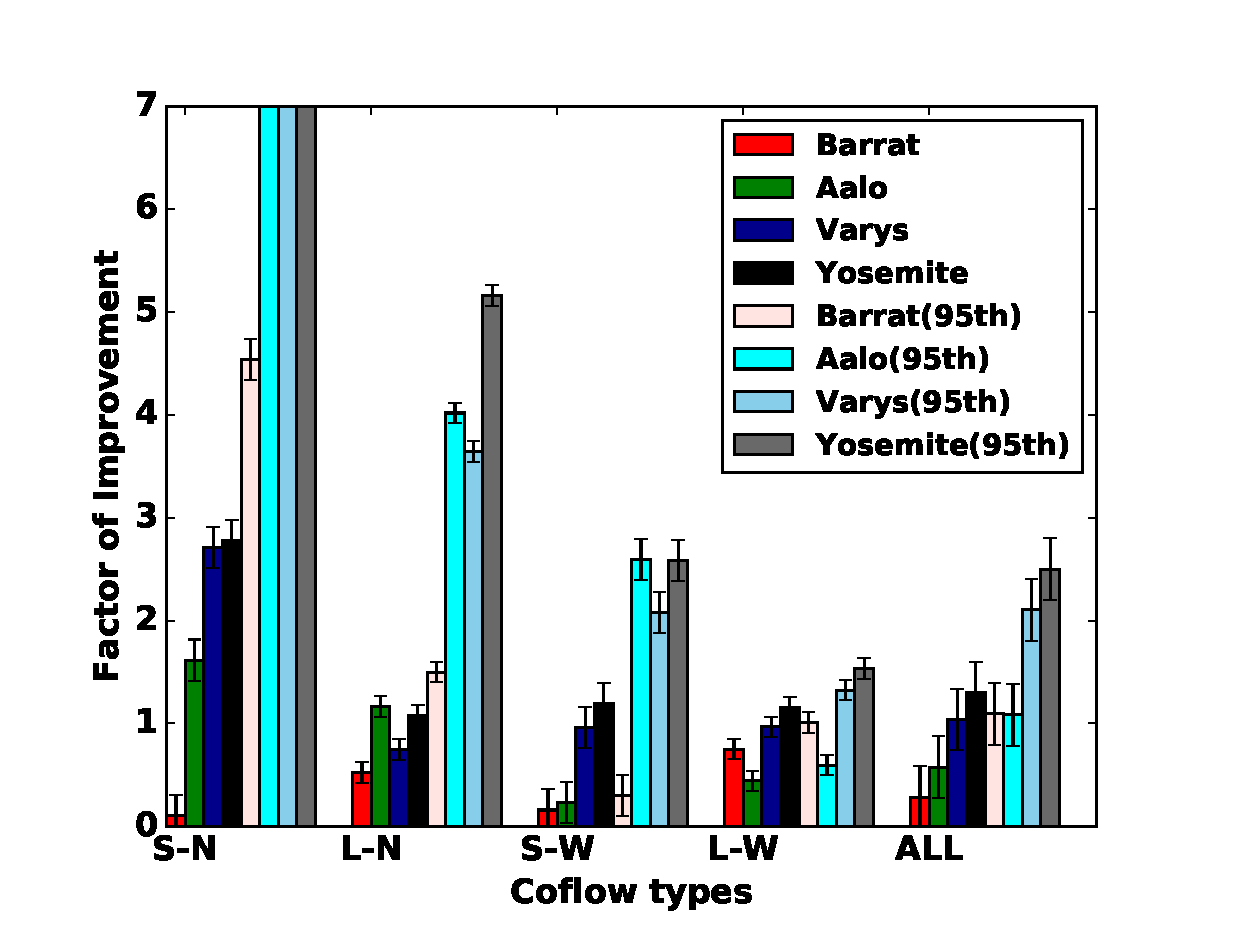
\includegraphics[width=0.5\columnwidth]{figures/Yosemite/figs/evaluation/ex2/weight_real_type.eps}}%
  \subcaptionbox{WCCT 分布}
      {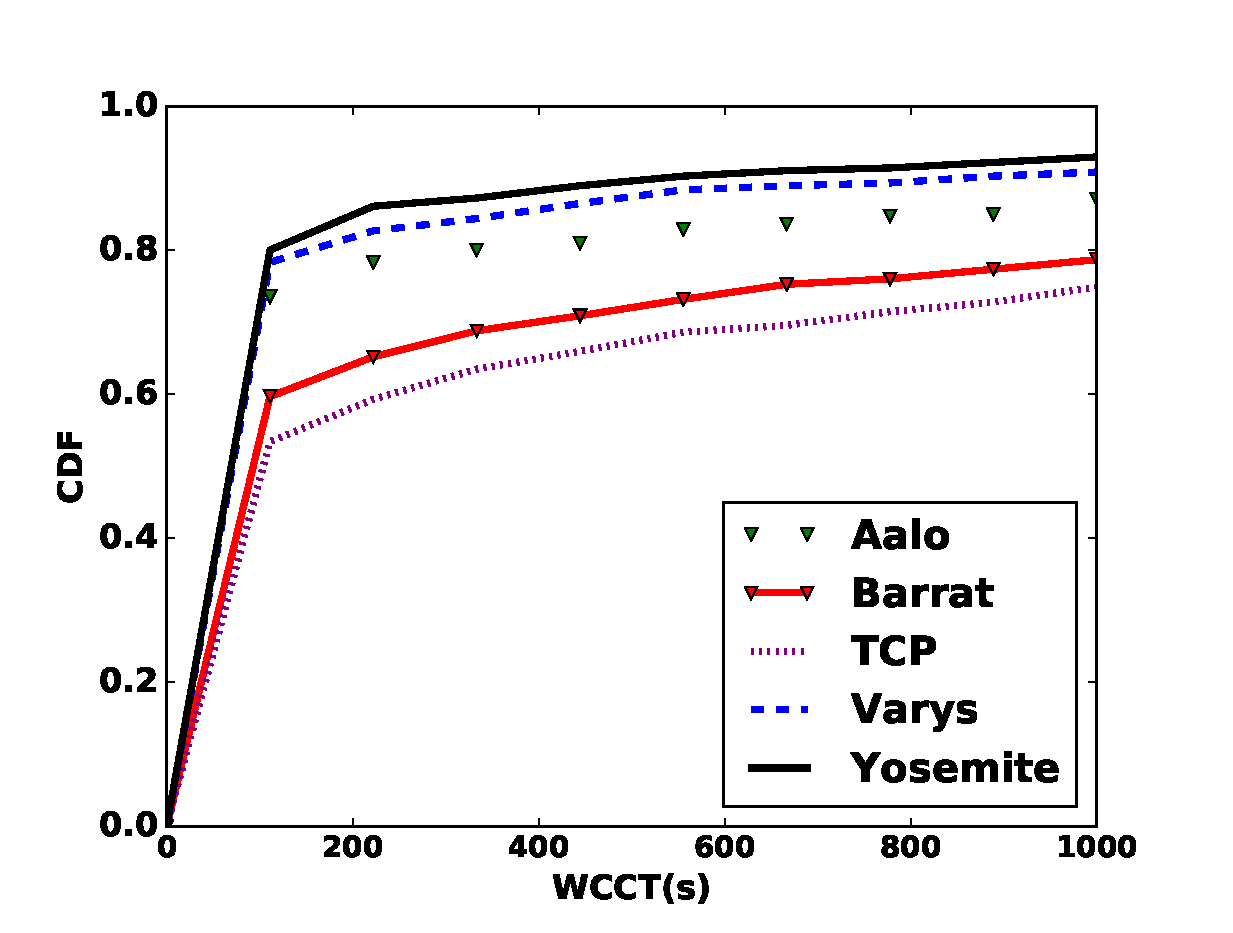
\includegraphics[width=0.5\columnwidth]{figures/Yosemite/figs/evaluation/ex2/weight_CDF_compare.eps}}
  \subcaptionbox{平均CCT}%标题的长度,超过则会换行,如下一个小图。
    {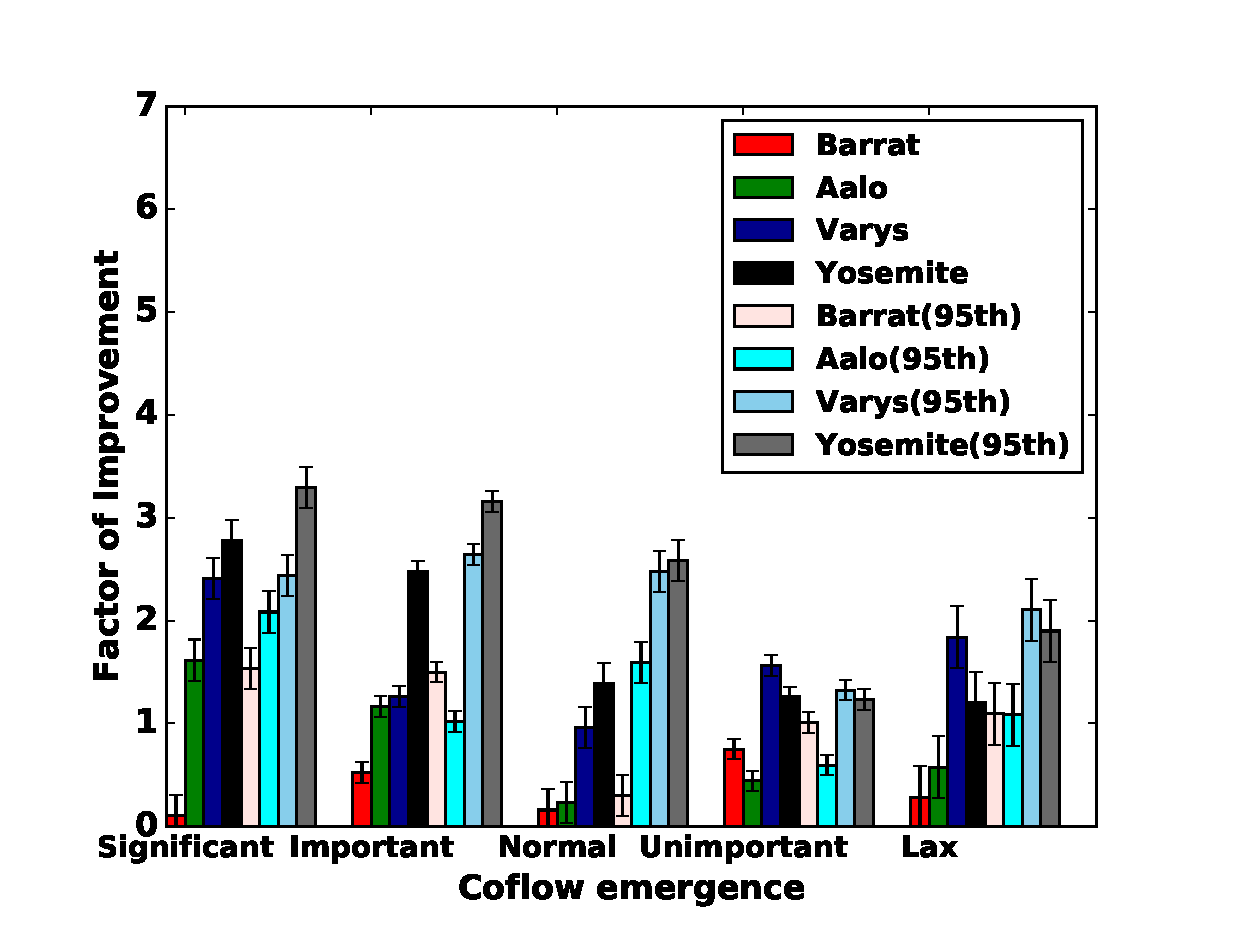
\includegraphics[width=0.5\columnwidth]{figures/Yosemite/figs/evaluation/ex2/nfake1.eps}}%
  %\hspace{7em}%
  \subcaptionbox{CCT分布}
      {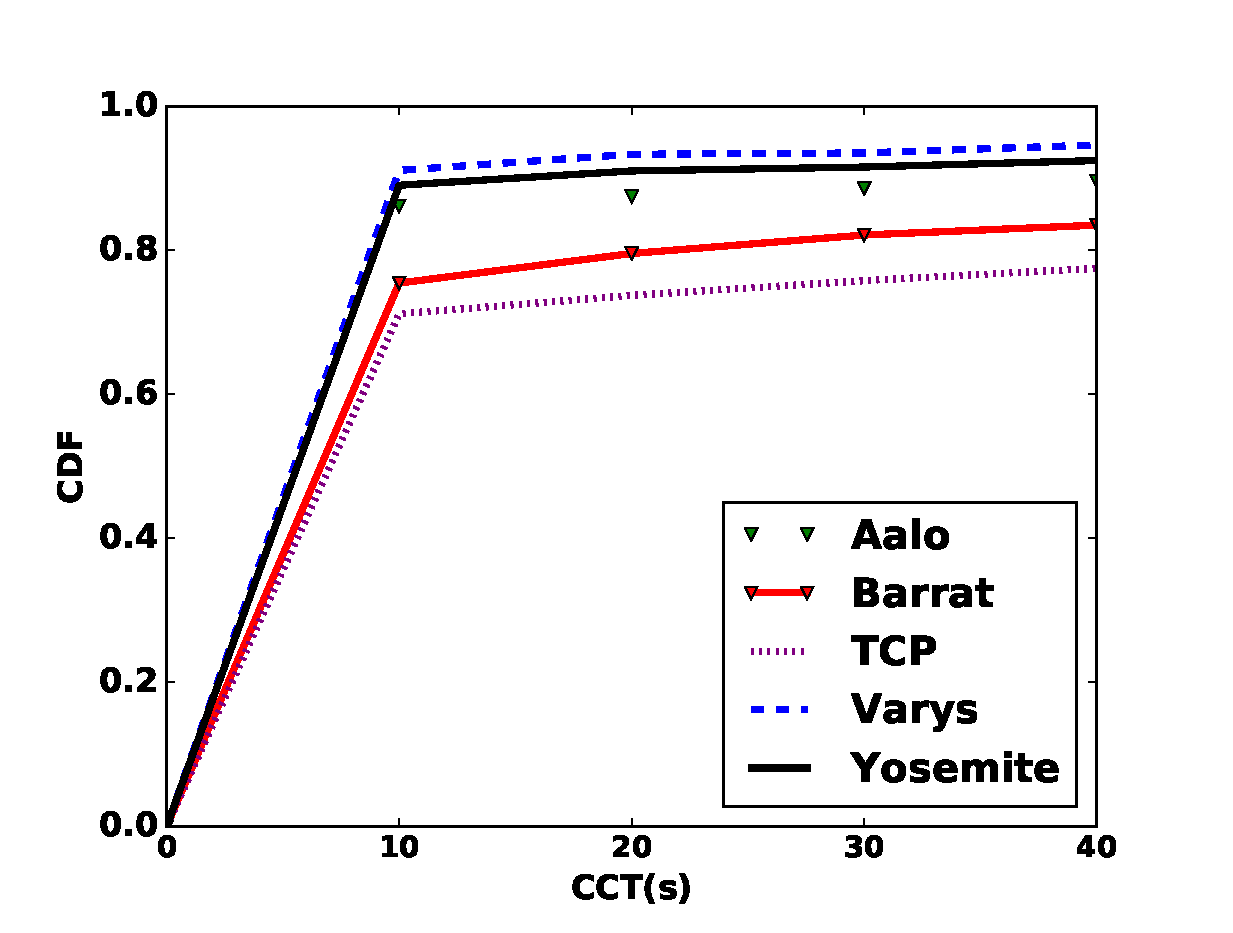
\includegraphics[width=0.5\columnwidth]{figures/Yosemite/figs/evaluation/ex2/CDF_compare.eps}}
  \caption{[仿真] 使用facebook 数据,平均WCCT和平均CCT,TCP被当作基准}
  \label{Yosemite-evaluation_facebook_fig}
\end{figure}

本部分使用facebook \cite{chowdhury2014efficient}的流量来测试Yosemite的性能。
Facebook的原始的数据并不包含权重信息,因此实验中随机给coflow在1,2,3,4,5中选择权重进行赋值。
因为权重是随机产生的,因此,每组实验重复100次,来避免随机产生权重带来的偶然影响。
实验图中绘制了error bar,同时标记了最大值,最小值以及平均值。
为了消除一些极值的影响,考虑更一般化的情形,在每组中,同时删除最前和最后$2.5\%$结果,
在实验中同时绘制了$95\%$的情形。

图\ref{Yosemite-evaluation_facebook_fig}(a)显示的是Yosemite对WCCT优化的结果,发现Yosemite对平均WCCT优化的性能是最好的。
Yosemite对于TCP性能提高的倍数为3.5$\times$(N-S),1.6$\times$(N-L),1.7$\times$(W-S),1.4$\times$(W-L)和1.5$\times$(ALL)。
使用Varys ,各个类型的coflow对于TCP性能提高的倍数为2.4$\times$(N-S),0.9$\times$(N-L),1.2$\times$(W-S),1.3$\times$(W-L)和1.2$\times$(ALL)。
而Aalo对于TCP性能提高的倍数为1.6$\times$(N-S),1.2$\times$(N-L),0.3$\times$(W-S),0.6$\times$(W-L)和0.8$\times$(ALL)。
使用Barrat,各个类型的coflow对于TCP性能提高的倍数为0.4$\times$(N-S),0.8$\times$(N-L),0.2$\times$(W-S),0.8$\times$(W-L)和0.4$\times$(ALL)。

为了避免一些极端情况对平均性能的影响,图\ref{Yosemite-evaluation_facebook_fig}(a)同时显示了$95\%$的实验结果。
使用Yosemite,各个类型的coflow对于TCP性能提高的倍数为25$\times$(N-S),5.5$\times$(N-L),2.5$\times$(W-S),1.5$\times$(W-L)和2.5$\times$(ALL)。
使用Varys ,各个类型的coflow对于TCP性能提高的倍数为22$\times$(N-S),4.5$\times$(N-L),2.1$\times$(W-S),1.2$\times$(W-L)和2.1$\times$(ALL)。
使用Aalo,各个类型的coflow对于TCP性能提高的倍数为15$\times$(N-S),4.1$\times$(N-L),2.5$\times$(W-S),0.5$\times$(W-L)和1.2$\times$(ALL)。
使用Barrat,各个类型的coflow对于TCP性能提高的倍数为4.5$\times$(N-S),1.6$\times$(N-L),0.2$\times$(W-S),1.2$\times$(W-L)和1.1$\times$(ALL)。


图\ref{Yosemite-evaluation_facebook_fig}(b)表示WCCT的分布。
可以看到,80%以上的Yosemite的WCCT在200s以内,而Varys,Aalo,Barrat的是70%,65%,60%。
Yosemite比Varys,Aalo和Barrat要好15%,25%,30%。


图\ref{Yosemite-evaluation_facebook_fig}(c)显示了具有不同紧急程度的coflows平均CCT。
可以看到Yosemite对于TCP性能提高的倍数是2.5$\times$(紧急),2.3$\times$(重要),1.2$\times$(正常),1.4$\times$(不重要),1.5$\times$(松散)。
Varys是2.2$\times$(紧急),1.5$\times$(重要),1.4$\times$(正常),1.6$\times$(不重要),1.9$\times$(松散)。
Aalo是1.2$\times$(紧急),1.4$\times$(重要),0.3$\times$(正常),0.6$\times$(不重要),0.7$\times$(松散)。
Barrat是1.4$\times$(紧急),1.2$\times$(重要),0.3$\times$(正常),0.8$\times$(不重要),0.8$\times$(松散)。
图\ref{Yosemite-evaluation_facebook_fig}(c)同时显示了95$\%$的情形,
对于95$\%$的场景,Yosemite对于TCP性能提高的倍数是3.2$\times$(重要),3.1$\times$(重要),2.9$\times$(正常),1.6$\times$(不重要),1.9$\times$(松散)。
Varys是2.2$\times$(紧急),2.1$\times$(重要),2.0$\times$(正常),1.9$\times$(不重要),2.3$\times$(松散)。
Aalo是1.5$\times$(紧急),1.2$\times$(重要),0.6$\times$(正常),0.8$\times$(不重要),0.7$\times$(松散)。
Barrat是0.2$\times$(紧急),0.6$\times$(重要),0.4$\times$(正常),0.8$\times$(不重要),0.5$\times$(松散)。
可以看到,Yosemite对于紧急的和重要的coflow的优化水平要比Varys好20%,
但对于重要性在正常以下的coflow(包含正常),Varys比Yosemite好20%。
这是因为当Varys调度coflows只考虑网络的情形,并没有把coflow的重要性考虑进去。
而Yosemite既考虑到网络条件,又考虑到coflows的重要性。
在Yosemite之下,紧急的和重要的coflow有更高的优先级,因此平均完成时间会缩短。

图\ref{Yosemite-evaluation_facebook_fig}(d)显示了不同方法下的CCT的分布。
Varys下80%以上CCT在20s以内,Yosemite,Aalo,Barrat分别为75%,65%,60%。
统计所有coflow的平均CCT,Varys比Yosemite的效果要好10%。
可以看到,Varys比Aalo,Barrat在平均CCT和平均WCCT最小化方面表现更好。
因此在下面的实验中,主要使用Varys作为参考方法来展示Yosemite的性能。

\subsection{使用中等规模的数据中心流量数据进行测试}

\begin{figure}[h]
  \centering%
  \subcaptionbox{平均WCCT} %标题的长度,超过则会换行,如下一个小图。
    {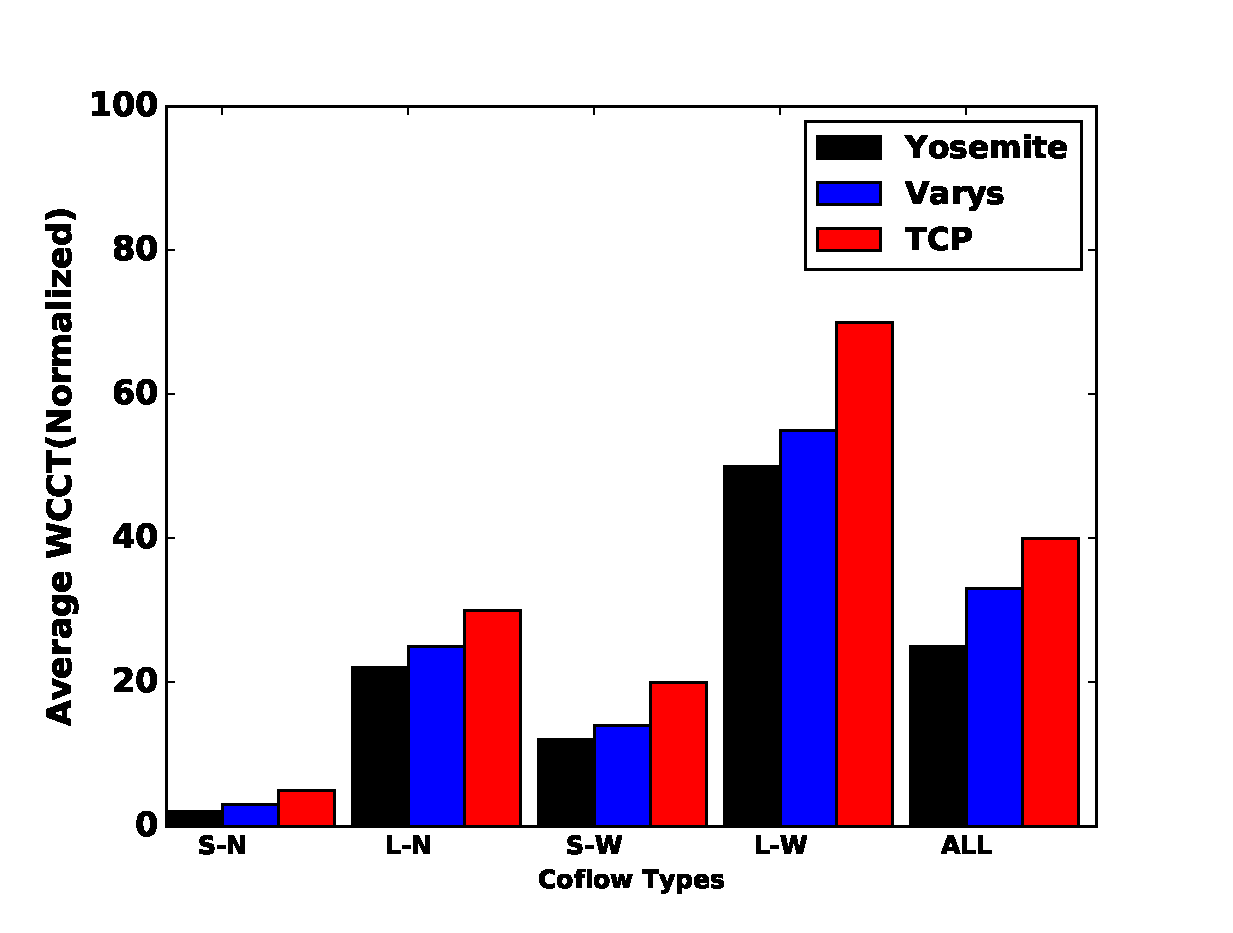
\includegraphics[width=0.5\columnwidth]{figures/Yosemite/figs/evaluation/ex1/evaluation_motivation1.eps}}%
  \subcaptionbox{平均CCT}
      {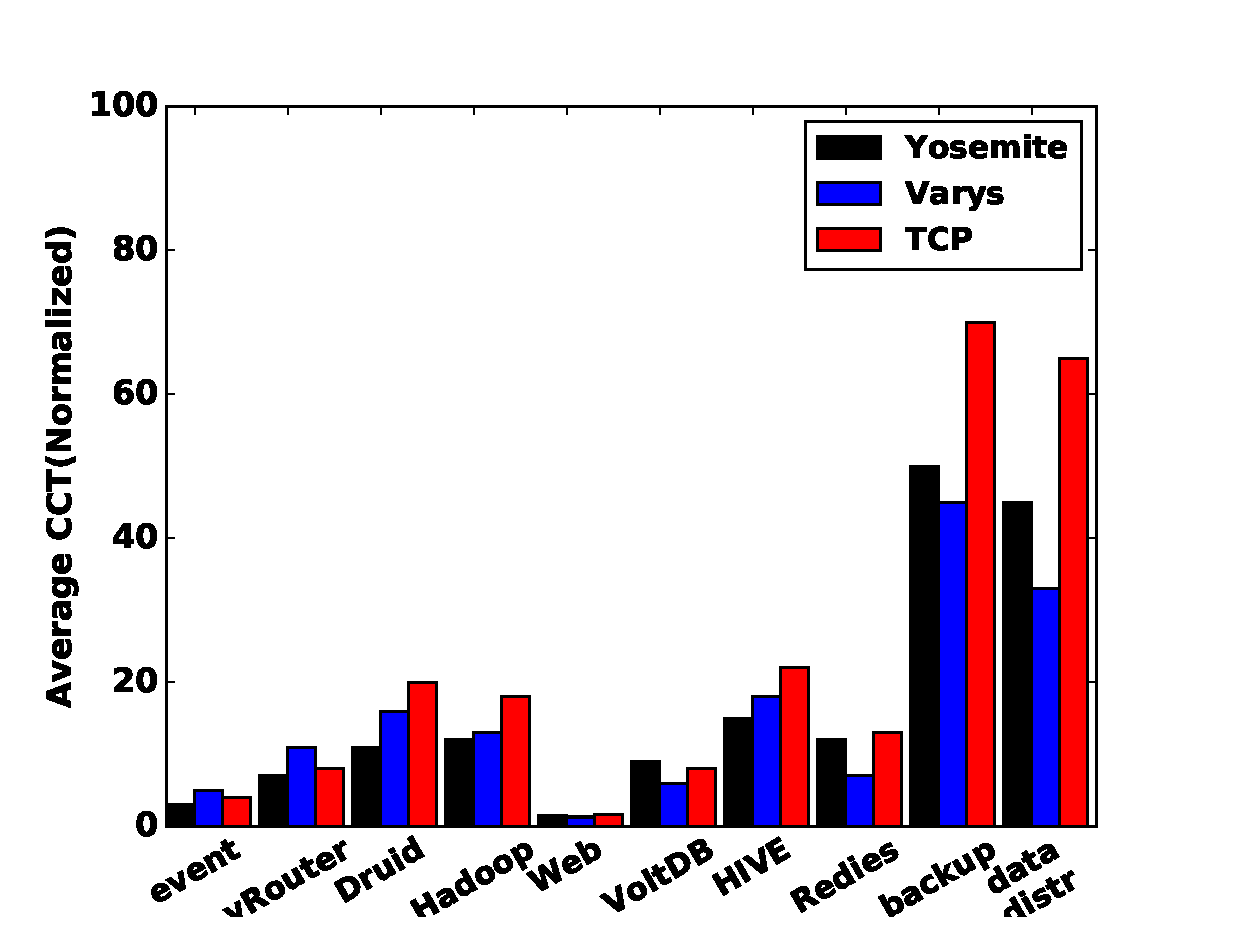
\includegraphics[width=0.5\columnwidth]{figures/Yosemite/figs/evaluation/ex1/evaluation_motivation2.eps}}
  \subcaptionbox{Hadoop WCCT}%标题的长度,超过则会换行,如下一个小图。
    {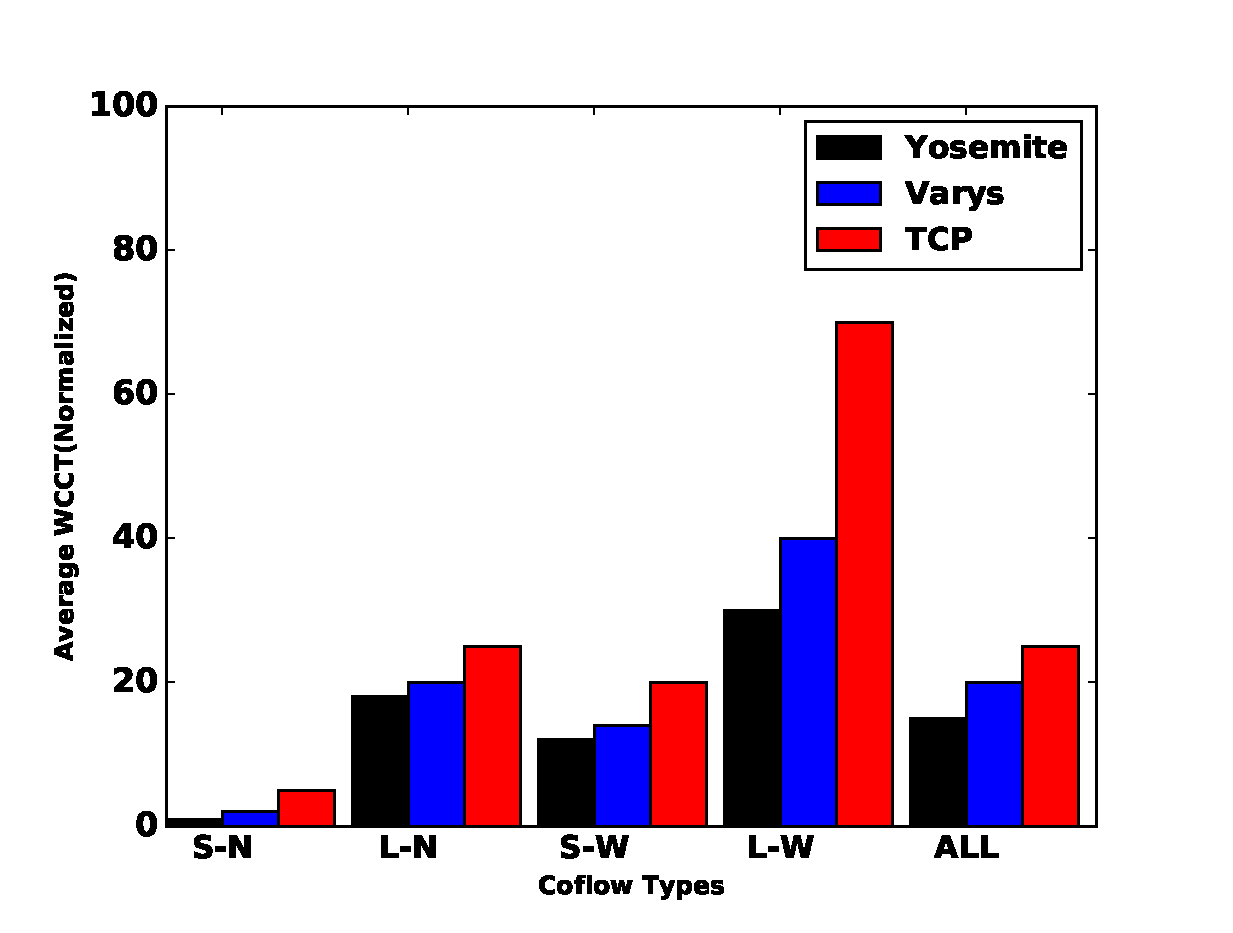
\includegraphics[width=0.5\columnwidth]{figures/Yosemite/figs/evaluation/ex1/evaluation_motivation3.eps}}%
  %\hspace{7em}%
  \subcaptionbox{Hadoop CCT}
      {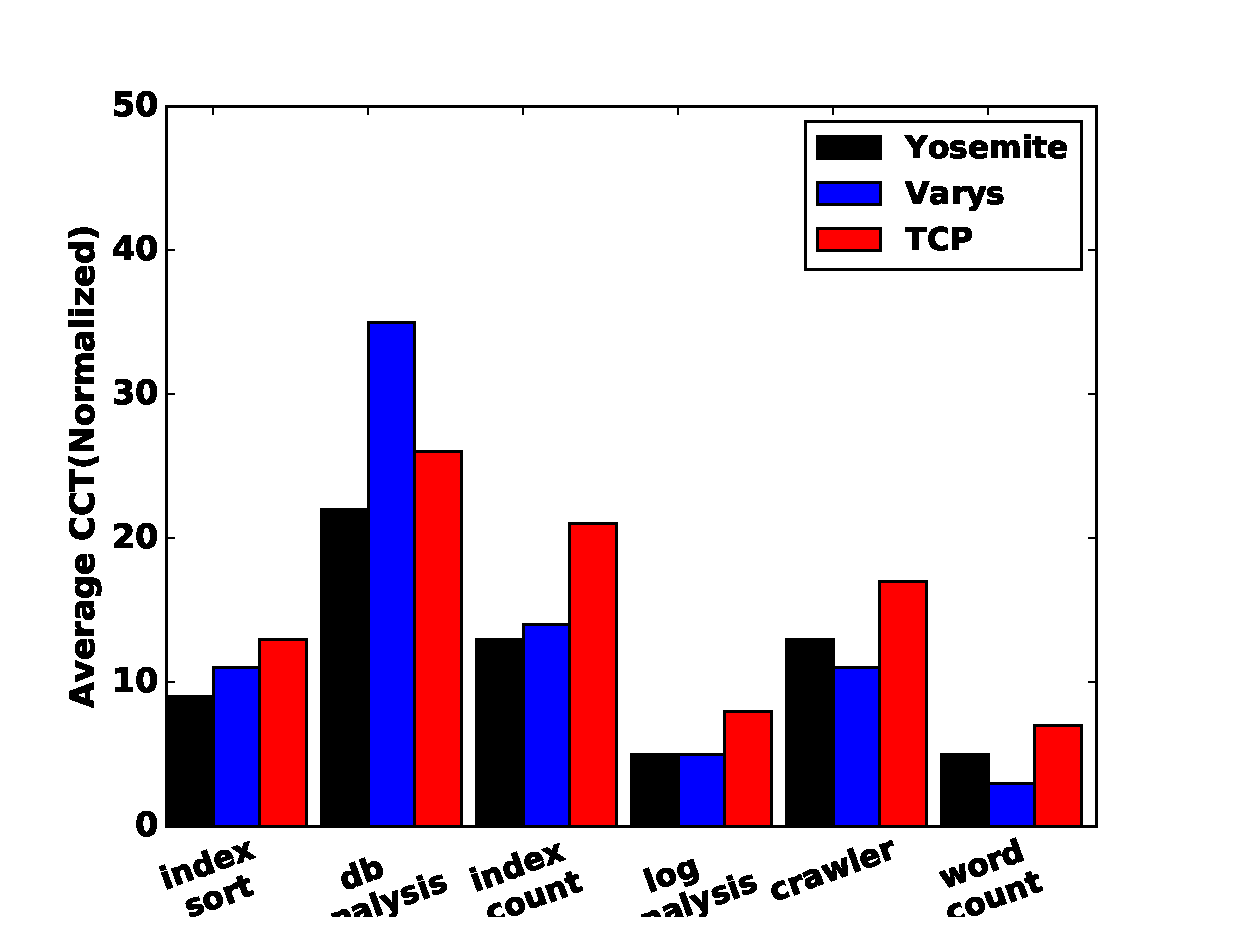
\includegraphics[width=0.5\columnwidth]{figures/Yosemite/figs/evaluation/ex1/evaluation_motivation4.eps}}
  \caption{[仿真]所有应用和hadoop的平均CCT(标准化)和平均。Varys忽略coflow的重要性,只考虑网络拥塞,Yosemite同时考虑coflow的重要性和网络拥塞}
  \label{Yosemite-evaluation_motivation_fig}
\end{figure}

在这个部分中,解决\ref{Yosemite-motivation}部分提出的问题。
在的中等规模的数据总心中,应用有5个优先级,紧急,重要,标准,不重要,松散。
使用5,4,3,2,1来表示这5个优先级。
图\ref{Yosemite-evaluation_motivation_fig}显示了实验结果。





图\ref{Yosemite-evaluation_motivation_fig}(a)显示了对所有coflows的平均WCCT。
发现Varys的平均WCCT是8 (Narrow\&Short), 20(Narrow\&Long), 15 (Wide\&Short), 40  (Wide\&Long) and 30(ALL)。
Yosemite的平均WCCT是5 (Narrow\&Short), 15(Narrow\&Long), 10 (Wide\&Short), 30  (Wide\&Long) and 20(ALL)。
对于最小化平均WCCT,Yosemite性能大约有20$\%$的性能提升。

从图\ref{Yosemite-evaluation_motivation_fig}(b),看到对于vRouter和event,这两个应用有紧急程度的应用,
Varys的性能表现和TCP基本相同,Yosemite比TCP性能提高20$\%$。
对于Hadoop和Druid,这两个应用的优先级是重要,Yosemite的性能比Varys高30$\%$。
对于其它的应用,Varys性能比Yosemite好10$\%$。

图\ref{Yosemite-evaluation_motivation_fig}(c)展示的是Hadoop 平均WCCT,
图\ref{Yosemite-evaluation_motivation_fig}(d)展示的是Hadoop CCT。
对于index sort和db analysis,这两种应用在数据中心中优先级属于重要的优先级,Vayrs性能甚至比TCP差。
然而,使用Yosemite,性能大约有30\%$\sim$ 40\%提升。
但是对于不重要和松散的coflows,Vayrs甚至性能更好。
对于平均WCCT,Yosemite性能比Varys有20\%性能提升。

\subsection{权重的讨论}

\begin{figure}[h]
\centering
\subcaptionbox{小wd}
 {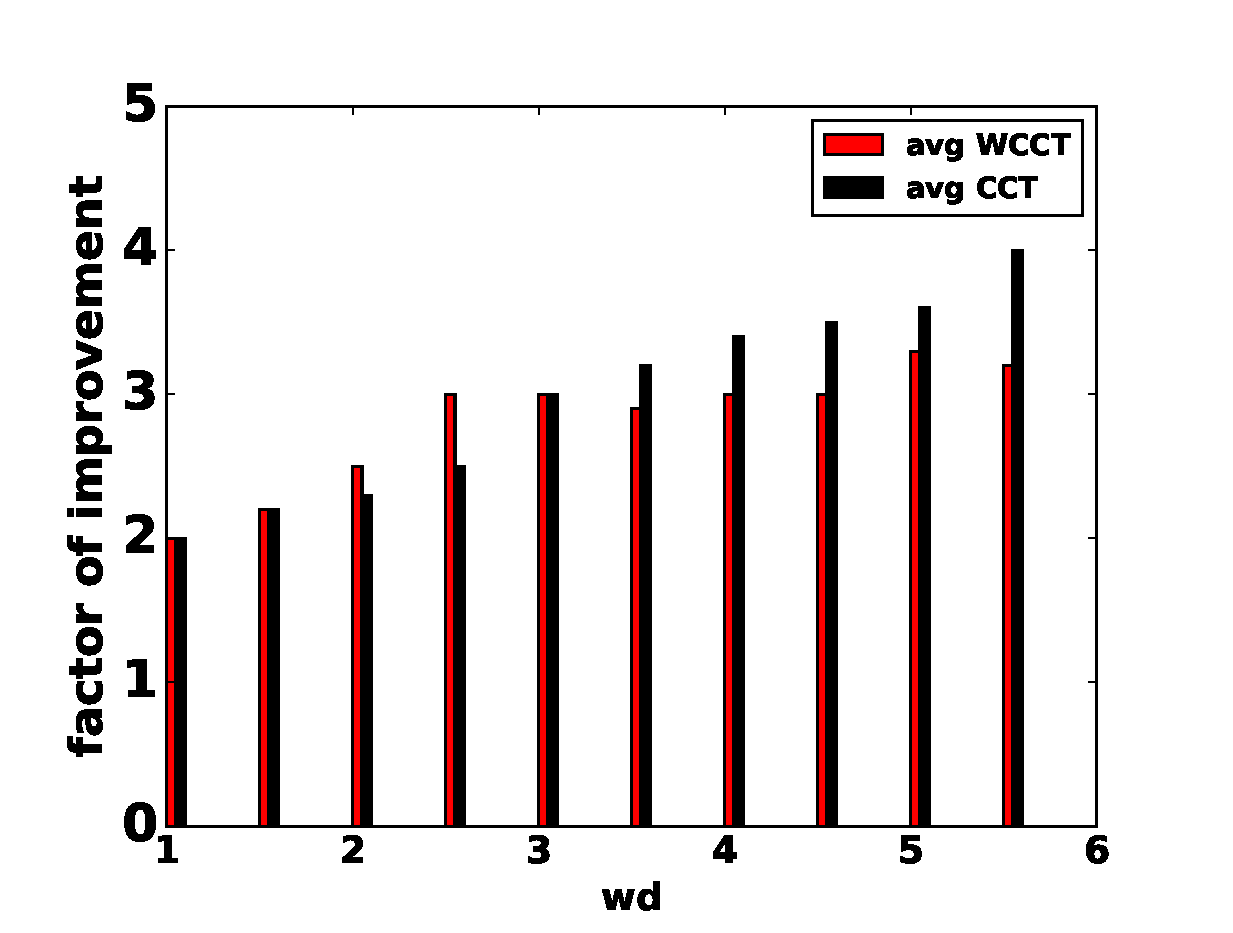
\includegraphics[width=0.48\columnwidth]{figures/Yosemite/figs/evaluation/ex3/fake7.eps}}
\subcaptionbox{大wd}
{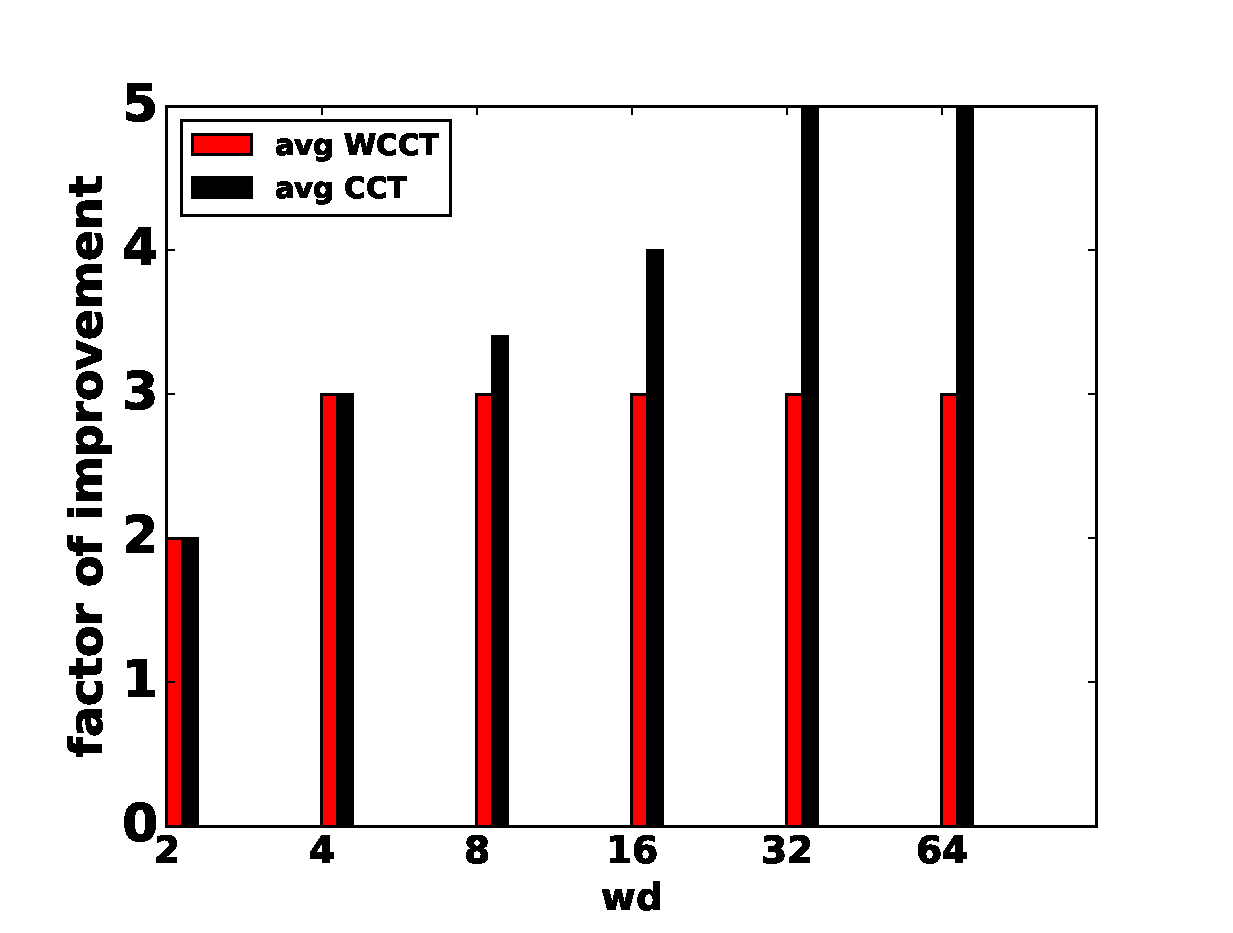
\includegraphics[width=0.48\columnwidth]{figures/Yosemite/figs/evaluation/ex3/fake8.eps}}
\caption{[仿真] 不同权重设置下的,平均WCCT和平均CCT,TCP被当做基准}
\label{Yosemite-evaluation_weight_fig}
\end{figure}

权重在Yosemite调度系统中有重要的作用,在上面的实验中,权重之间的差是1。
在这组实验中使用Facebook的流量,设置权重在1,1+wd,1+2*wd,1+3*wd,1+4*wd之间,改变wd从1到10,
图\ref{Yosemite-evaluation_weight_fig}(a)显示了平均WCCT相对于TCP提高的比例,重要coflow($weight> 1+2*wd$)的平均CCT相对于TCP提高的比例。
可以看到随着权重差异的增加,平均WCCT的提高幅度从2增加到2.8,但是对于重要coflow的平均CCT提高幅度基本保持不变。
原因是Yosemite使用权重和已经发送数据流的大小作为排序因子,随着权重差异的增加,权重扮演的角色越来越大,因此重要的coflow排序在前,所以优先获得更多的网络资源,进而先传输完成。
图\ref{Yosemite-evaluation_weight_fig}(b)展示的是更大的wd差异值,wd从2增大到64,看到当wd $>$ 8时,重要性高得coflow提高变小,这和图\ref{Yosemite-evaluation_weight_fig}(a)的结果基本类似。

在实际中,权重的设置可以根据网络管理员的需求来进行决定,
当管理员认为coflow的紧急程度是十分重要的因子时,可以用比较大的wd,
当管理员认为网络拥塞情形和coflow的重要性同等重要时,
可以使用小的wd。



\subsection{策略和最优策略的差距}
\begin{figure}[b]
\begin{center}
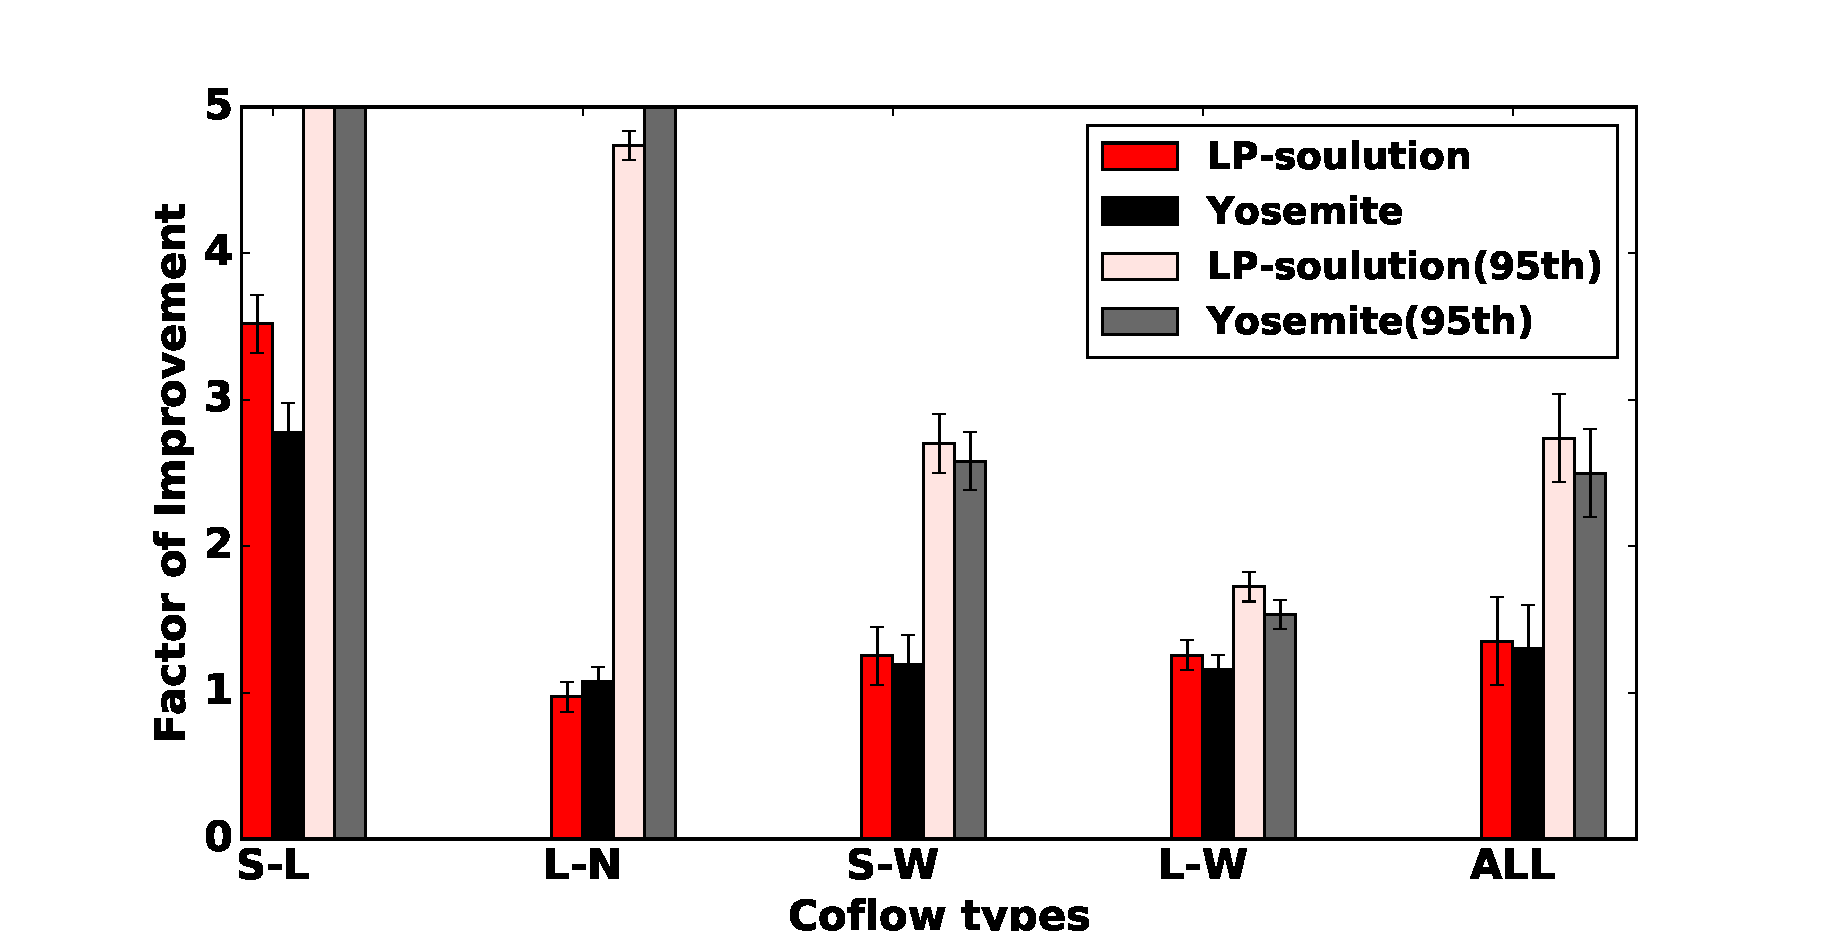
\includegraphics [width=0.8\columnwidth] {figures/Yosemite/figs/fake/fake1.eps}
\caption{[仿真] LP-based的策略和Yosemite策略性能对比}
\label{Yosemite-LP-based-fig}
\end{center}
\end{figure}
找到IWCCM问题的最优解很困难,但是找到了一个LP-based的策略\cite{qiu2015minimizing} ,这个算法的近似度为$\frac{67}{3}$,
用LP-based策略和Yosemite策略进行对比。
使用facebook的流量,并且从1,2,3,4,5随机的给coflow设置权重,重复这个实验20次,图 \ref{Yosemite-LP-based-fig}显示了实验结果。
看到,Yosemite相对于TCP提高程度为3.5 (Narrow\&Short), 1 (Narrow\&Long), 1.2 (Wide\&Short), 1.1 (Wide\&Long) and 1.1 (ALL),
LP-based的方法的提高幅度为 0.9 (Narrow\&Long), 1.3 (Wide\&Short), 1.3 (Wide\&Long) and 1.2 (ALL)。
发现,相对于LP-based的方法,Yosemite存在平均10\%的性能损失。

\subsection{在线策略和离线策略的差距}

\begin{figure}[h]
\centering 
\subcaptionbox{平均WCCT}
 {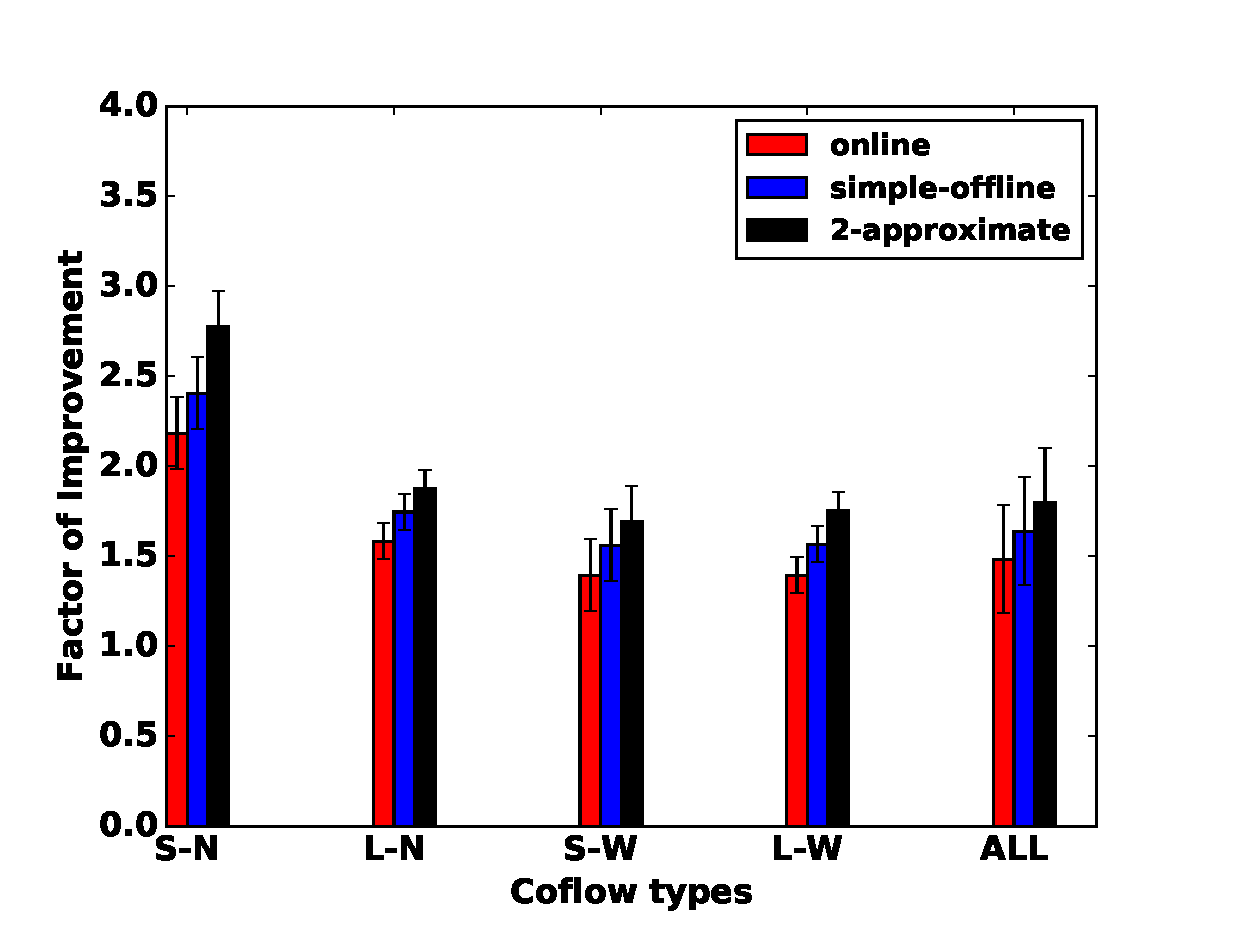
\includegraphics[width=0.32\columnwidth]{figures/Yosemite/figs/performance/nfake5.eps}}
\subcaptionbox{平均CCT}
{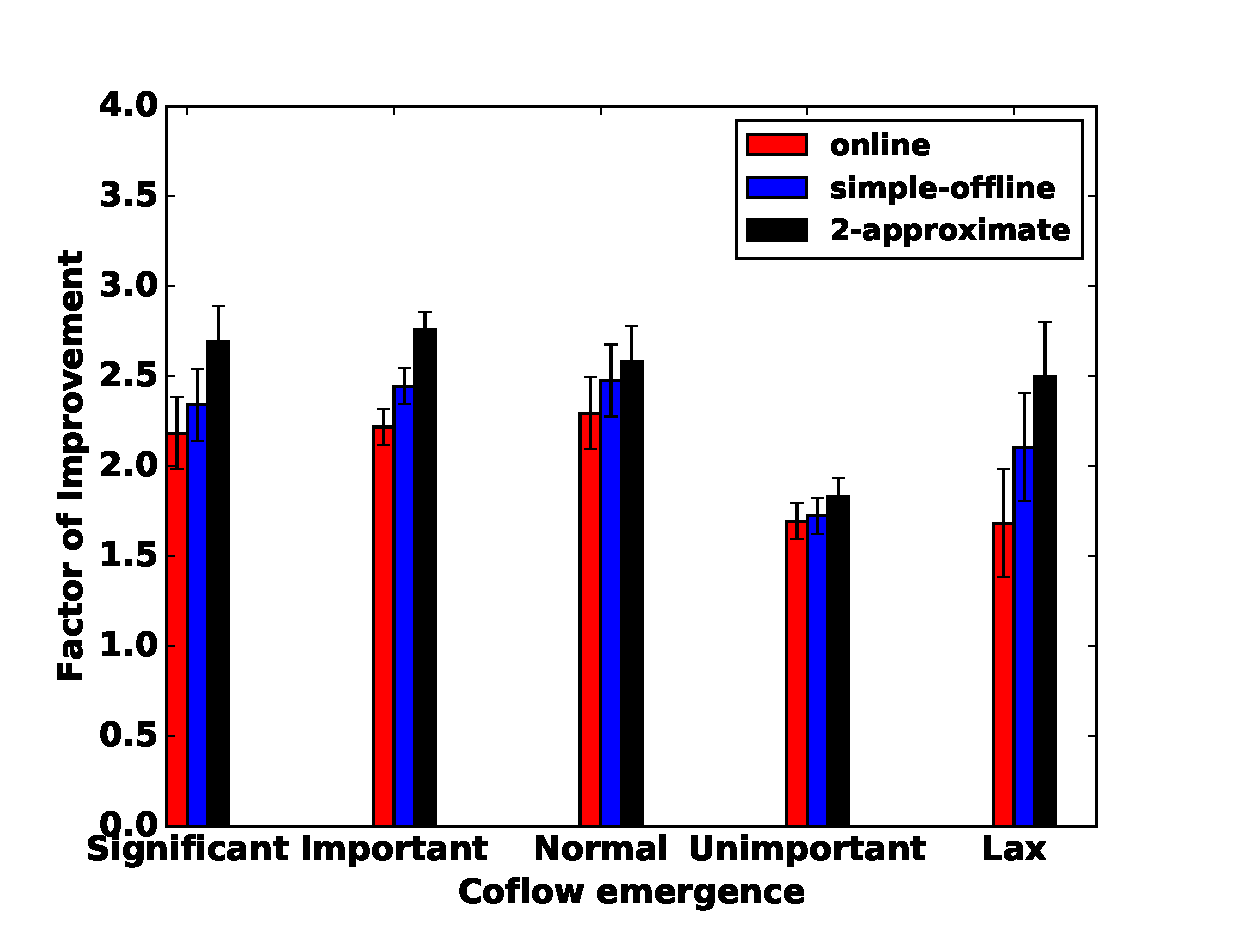
\includegraphics[width=0.32\columnwidth]{figures/Yosemite/figs/performance/nfake4.eps}}
\subcaptionbox{CCT的分布}
{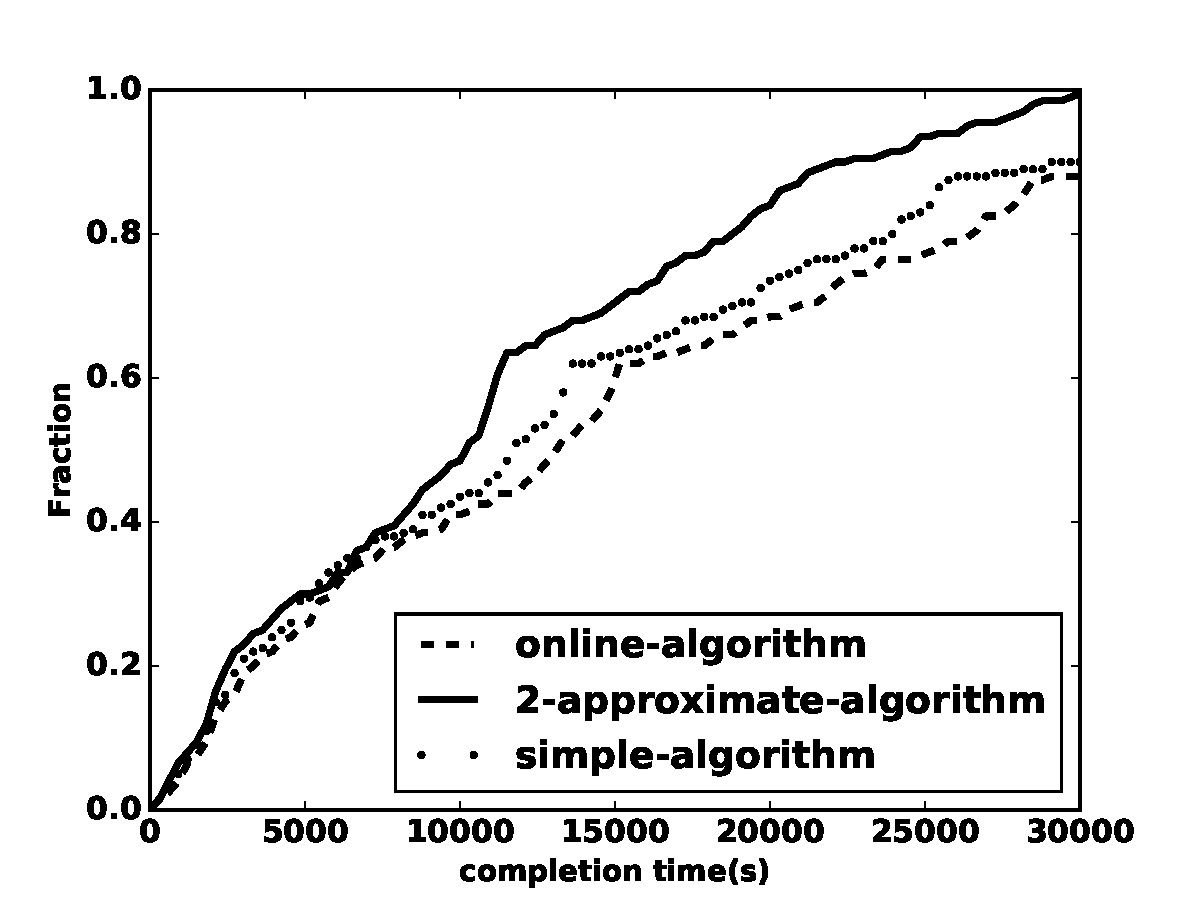
\includegraphics[width=0.32\columnwidth]{figures/Yosemite/figs/performance/online_offline.pdf}}
\caption{[仿真] 在线策略和离线策略对比,TCP被选作基准}
\label{Yosemite-evaluation_diff_fig}
\end{figure}

\begin{table}[h]
\centering
\footnotesize
          \caption{三个策略的对比} \label{tab-Yosemite-comparison}
          \begin{tabular}{|c|c|c|c|c|c|} \hline
              \toprule
              策略  &方式 & 复杂性 & 性能 &是否需要提前预知信息\\
              \midrule
              2-approximate & 离线    & 复杂     & 高 &需要\\
              \toprule
             simple-offline & 离线     & 简单     & 高& 需要 \\
             \toprule
            Yosemite & 在线    & 简单     & 高 & 不需要\\
              \bottomrule
          \end{tabular}
      \end{table}
      
事实上,在Yosemite策略中使用了两个放缩来简化策略,简单的离线策略假设数据中心中在每个端口上已经进行了负载均衡。
在线算法进一步假设长的coflow因为持续的时间长,因该有较低的优先级。
这两个放缩会损伤策略的性能。
为了展示策略性能的损失,假设在60台机器的小型数据中心有100条coflow,这些coflow同时在t=0启动,并且设置权重在1,2,3,4,5中随机选取。
重复每组实验100次,图\ref{Yosemite-evaluation_diff_fig}显示了实验结果。
注意,在实验中,error bar包含平均,最大和最小值。
从图\ref{Yosemite-evaluation_diff_fig}(a)看到,对于在线策略,WCCT相对于TCP提高倍数是1.6$\times$,
简单离线策略是1.7$\times$,2-近似策略是1.8$\times$。
和2-近似策略相比,对于优化平均WCCT,在线策略大约有10\%的性能损失。
图\ref{Yosemite-evaluation_diff_fig}(b)显示的是不同紧急程度的coflow性能对比。
看到在线策略,对于紧急和重要的coflow,平均提高幅度是2$\times$和2.1$\times$,简单离线策略提高幅度是2.2$\times$和2.3$\times$。
2-近似策略提高幅度是2.5$\times$,2.6$\times$。
这启示在线策略大约有30\%的性能损失。
图 \ref{Yosemite-evaluation_diff_fig}(c) 展示了CCT的分布情形。
发现对于2-近似策略有超过 80\% 的CCT在20000s以内,对于简单离线策略和在线策略是70\% 和 60\%。
表\ref{tab-Yosemite-comparison}展示的是不同策略的对比情形。
可以发现,在线策略有一些性能损失,但是在线策略,不需要预先得知流的长度。
因为在真实的环境中,一些应用的流的信息是无法预先得知的,
因此,不需要预先知道流信息的在线策略应用范围更广。


\section{本章小结}
本章中提出了基于重要性和网络拥塞的任务传输调度方案-Yosemite,
在不用预先得知流大小的前提下对coflow进行调度,
测量并分析AT\&T的流量,并把AT\&T的应用根据优先级进行区分。
最后,使用Facebook和AT\&T的流量对Yosemite性能进行评估。


